\documentclass[11pt]{beamer}
\usepackage[orientation=landscape,size=custom,width=16,height=9,scale=0.5,debug]{beamerposter} 
\usepackage[latin1]{inputenc}
\usepackage[utf8]{inputenc}
\usepackage[T1]{fontenc}

\usepackage{lmodern}
%\usefonttheme{serif}
%\usepackage[default, osfigures]{opensans}
\usepackage[sfdefault]{FiraSans}
\usepackage[dvipsnames,table,xcdraw]{xcolor}

\usepackage{url}
\usepackage{graphicx}
\usepackage{babel}
\usepackage{amsmath,amsfonts,amssymb} %%maths
\usetheme{Boadilla}
\usepackage{hyperref}
\usepackage{multirow}
\usepackage{longtable}
\usepackage{tabularx}
\usepackage{rotating}
\usepackage{siunitx}
\usepackage{multirow}
\usepackage{array} 
\usepackage{booktabs}
\newcommand{\head}[1]{\textnormal{\textbf{#1}}}
\usepackage{subfig}



\usepackage{caption}
\usepackage{subcaption}

\usepackage{listings}
%\usepackage{xcolor}
\definecolor{codegreen}{rgb}{0,0.6,0}
\definecolor{codegray}{rgb}{0.5,0.5,0.5}
\definecolor{codepurple}{rgb}{0.58,0,0.82}
\definecolor{backcolour}{rgb}{0.95,0.95,0.92}

\lstdefinestyle{mystyle}{
	backgroundcolor=\color{backcolour},   
	commentstyle=\color{codegreen},
	keywordstyle=\color{magenta},
	numberstyle=\tiny\color{codegray},
	stringstyle=\color{codepurple},
	basicstyle=\ttfamily\footnotesize,
	breakatwhitespace=false,         
	breaklines=true,                 
	captionpos=b,                    
	keepspaces=true,                 
	numbers=left,                    
	numbersep=5pt,                  
	showspaces=false,                
	showstringspaces=false,
	showtabs=false,                  
	tabsize=2
}

\lstset{style=mystyle}


\usepackage{tikz}
\usetikzlibrary{spy}

\setbeamertemplate{section in toc}[circle]
\setbeamertemplate{itemize items}[default]
\setbeamertemplate{itemize subitem}[square]
\setbeamertemplate{itemize subsubitem}[circle]
\setbeamertemplate{itemize mini template}[ball]

\setbeamertemplate{enumerate items}[circle]
\setbeamertemplate{enumerate subitem}[square]
\setbeamertemplate{enumerate subsubitem}[circle]
\setbeamertemplate{enumerate mini template}[ball]


\renewcommand{\baselinestretch}{1.3}
\setbeamersize{text margin left=0.5cm}
\setbeamersize{text margin right=0.5cm}


\setbeamertemplate{navigation symbols}{}

\begin{document}
	\author[Nith Kosal]{Nith Kosal}
	\title[Presentation Title]{\textbf{Introduction to Data Science}}
	\subtitle{\textbf{Welcome and Motivation Session}}
	\titlegraphic{\includegraphics[width=0.2\linewidth]{Figure/Logo}}
	\institute{Future Forum}
	\date[\today]{Future Forum, April 9, 2022}
	%\subject{}
	%\setbeamercovered{transparent}
	%\setbeamertemplate{navigation symbols}{}
	\begin{frame}[plain]
		\maketitle
	\end{frame}
	

	%------------------------------------------------------------------%


	
	\begin{frame}

		\frametitle{Dataset Terminology}
		
		\begin{itemize}
			\item Data science is an exciting discipline that allows you to turn raw data into understanding, insight, and knowledge.
			\item We're going to learn to do this in a tidy way -- more on that later!
			\item This is a course on introduction to data science, with an emphasis on statistical thinking.
		\end{itemize}
	\end{frame}
	%------------------------------------------------------------------%
	
	
	\begin{frame}
		\section{Theoretical Model}
		\frametitle{Theoretical Model}
		
		\begin{figure}
			\subfloat[\centering MS Excel]{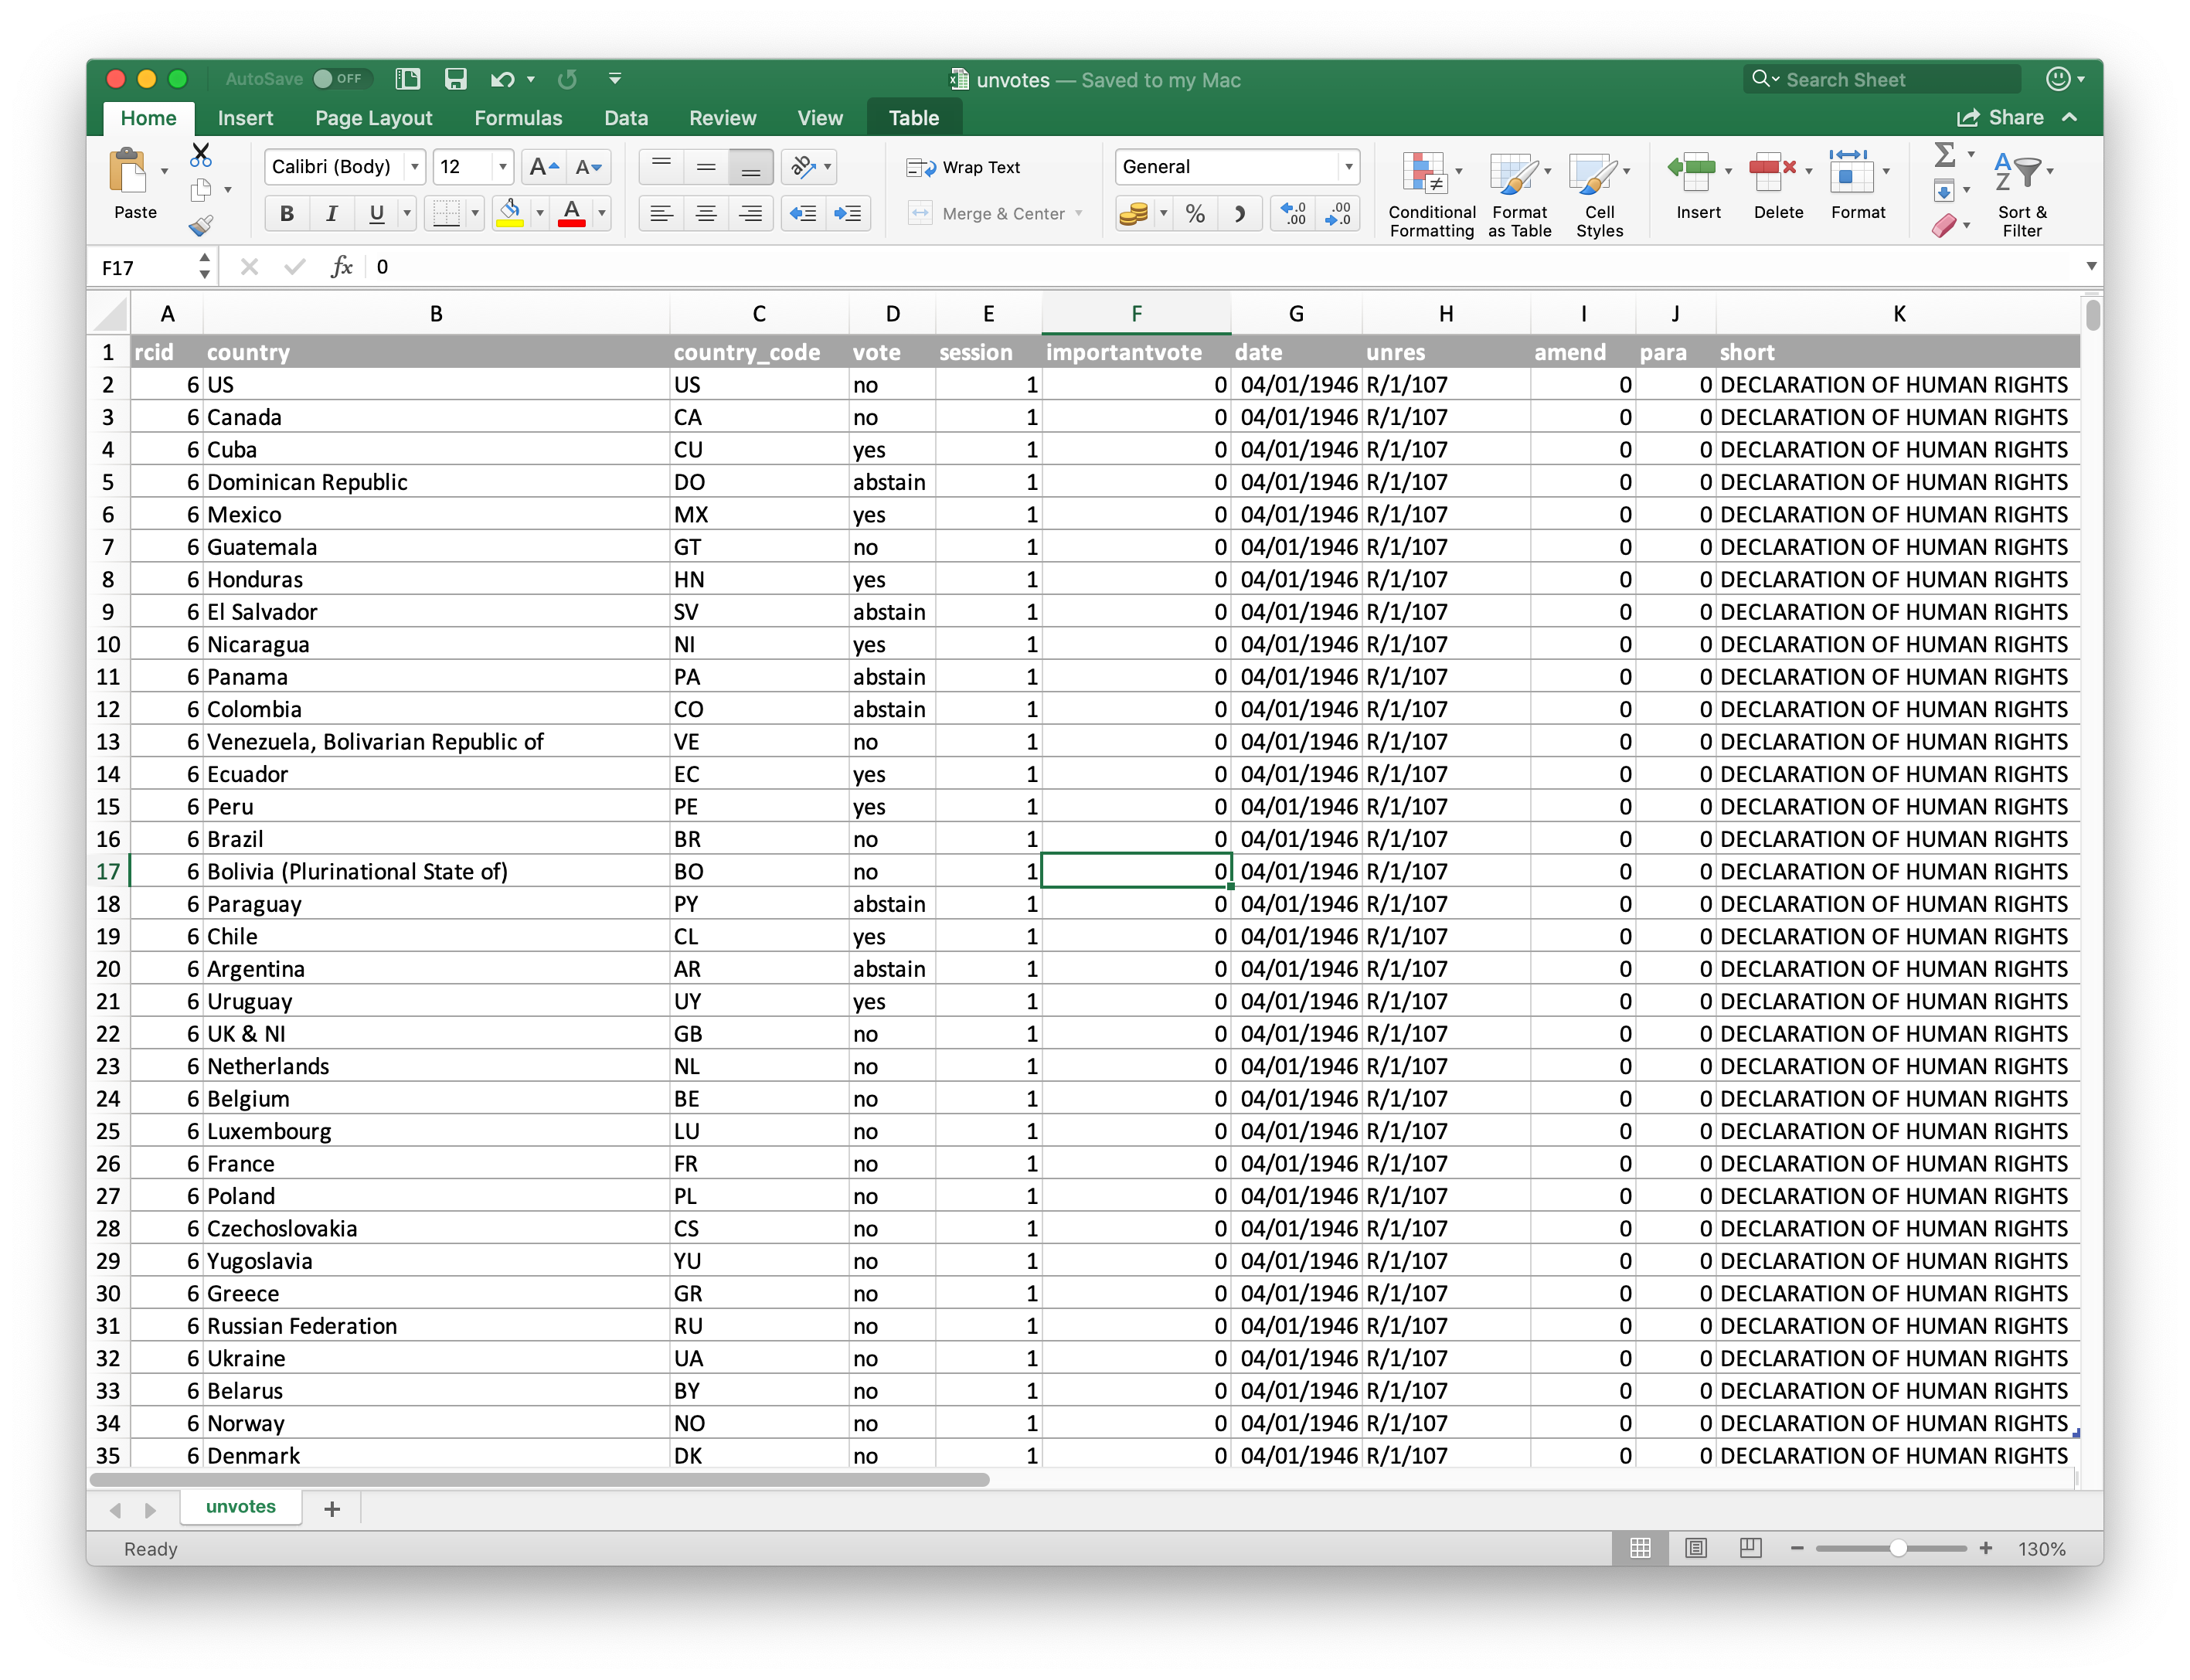
\includegraphics[trim=0cm 0cm 0cm 0cm, clip=true, totalheight=.6\textheight, angle=0]{Images/S1/excel}}
			\subfloat[\centering Stata]{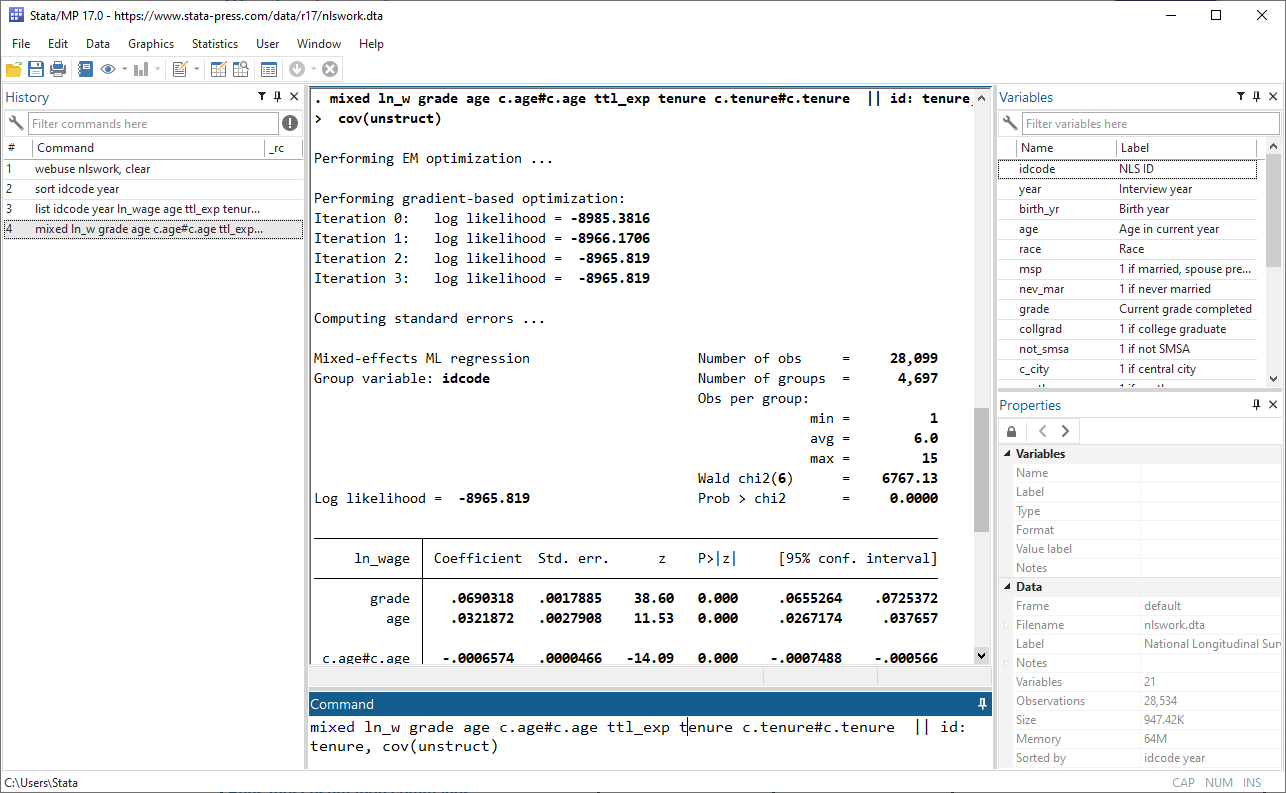
\includegraphics[trim=0cm 0cm 0cm 0cm, clip=true, totalheight=.59\textheight, angle=0]{Images/S1/stata}}
		\end{figure}
	
	\end{frame}
	%------------------------------------------------------------------%
	
	\begin{frame}
		\section{Empirical Framework}
		\frametitle{}

			\begin{figure}
				\vspace{0em}
				\subfloat[\centering RStudio]{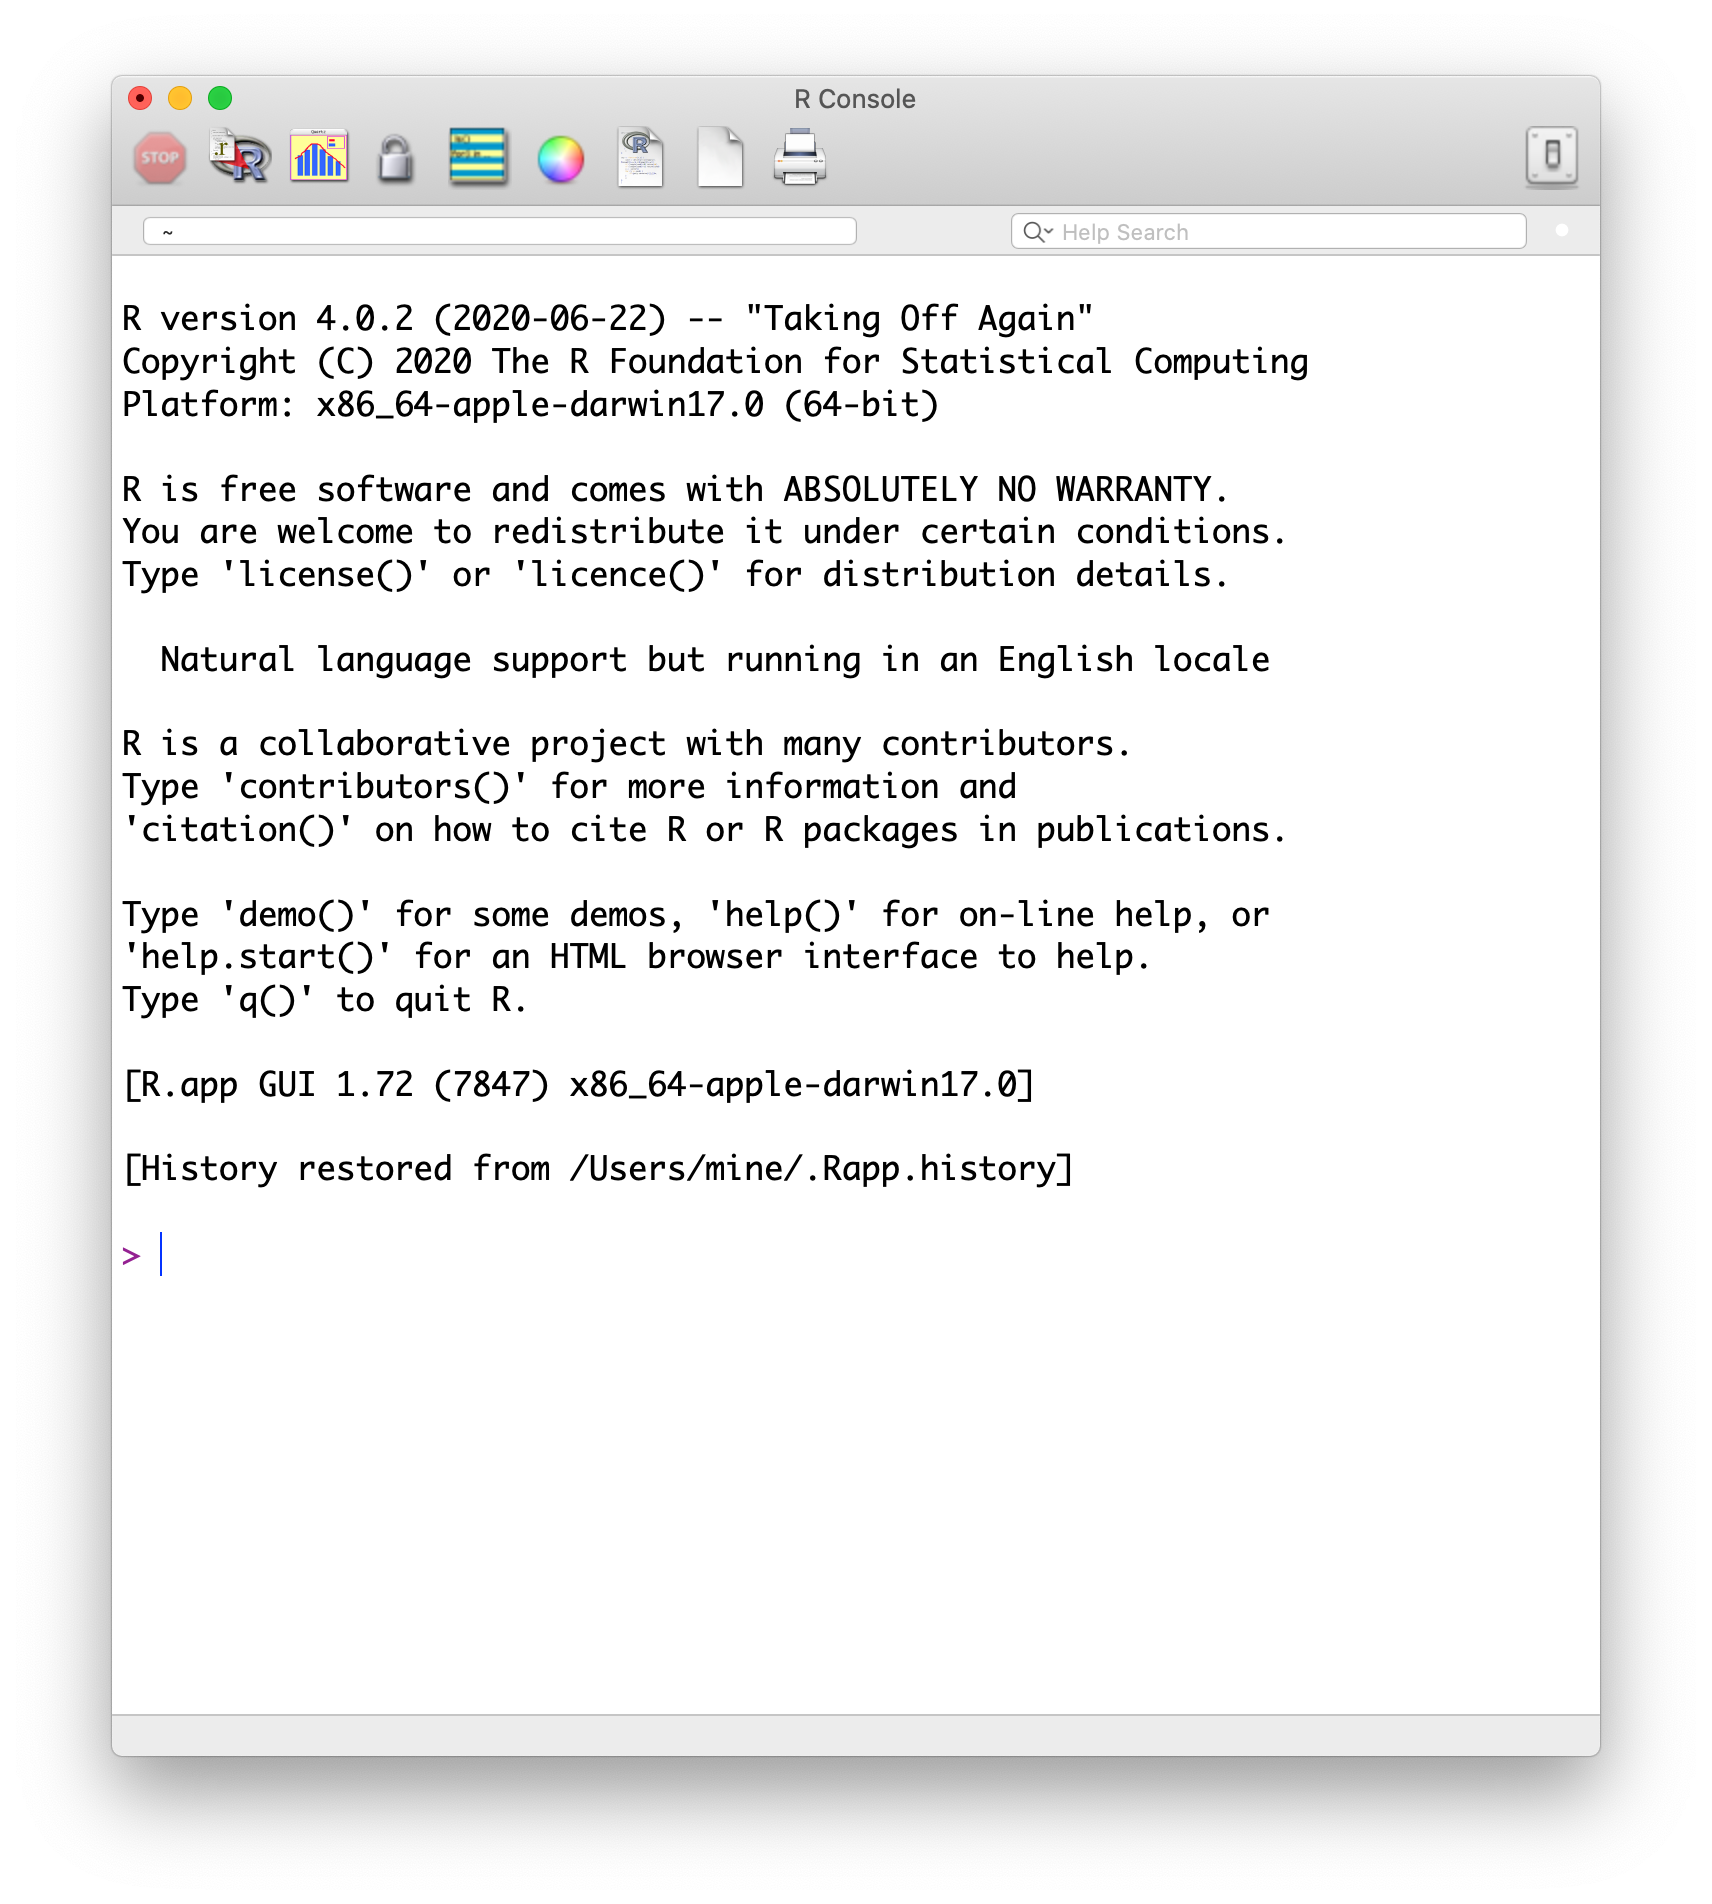
\includegraphics[trim=0cm 0cm 0cm 0cm, clip=true, totalheight=.8\textheight, angle=0]{Images/S1/r}}
				\subfloat[\centering RStudio]{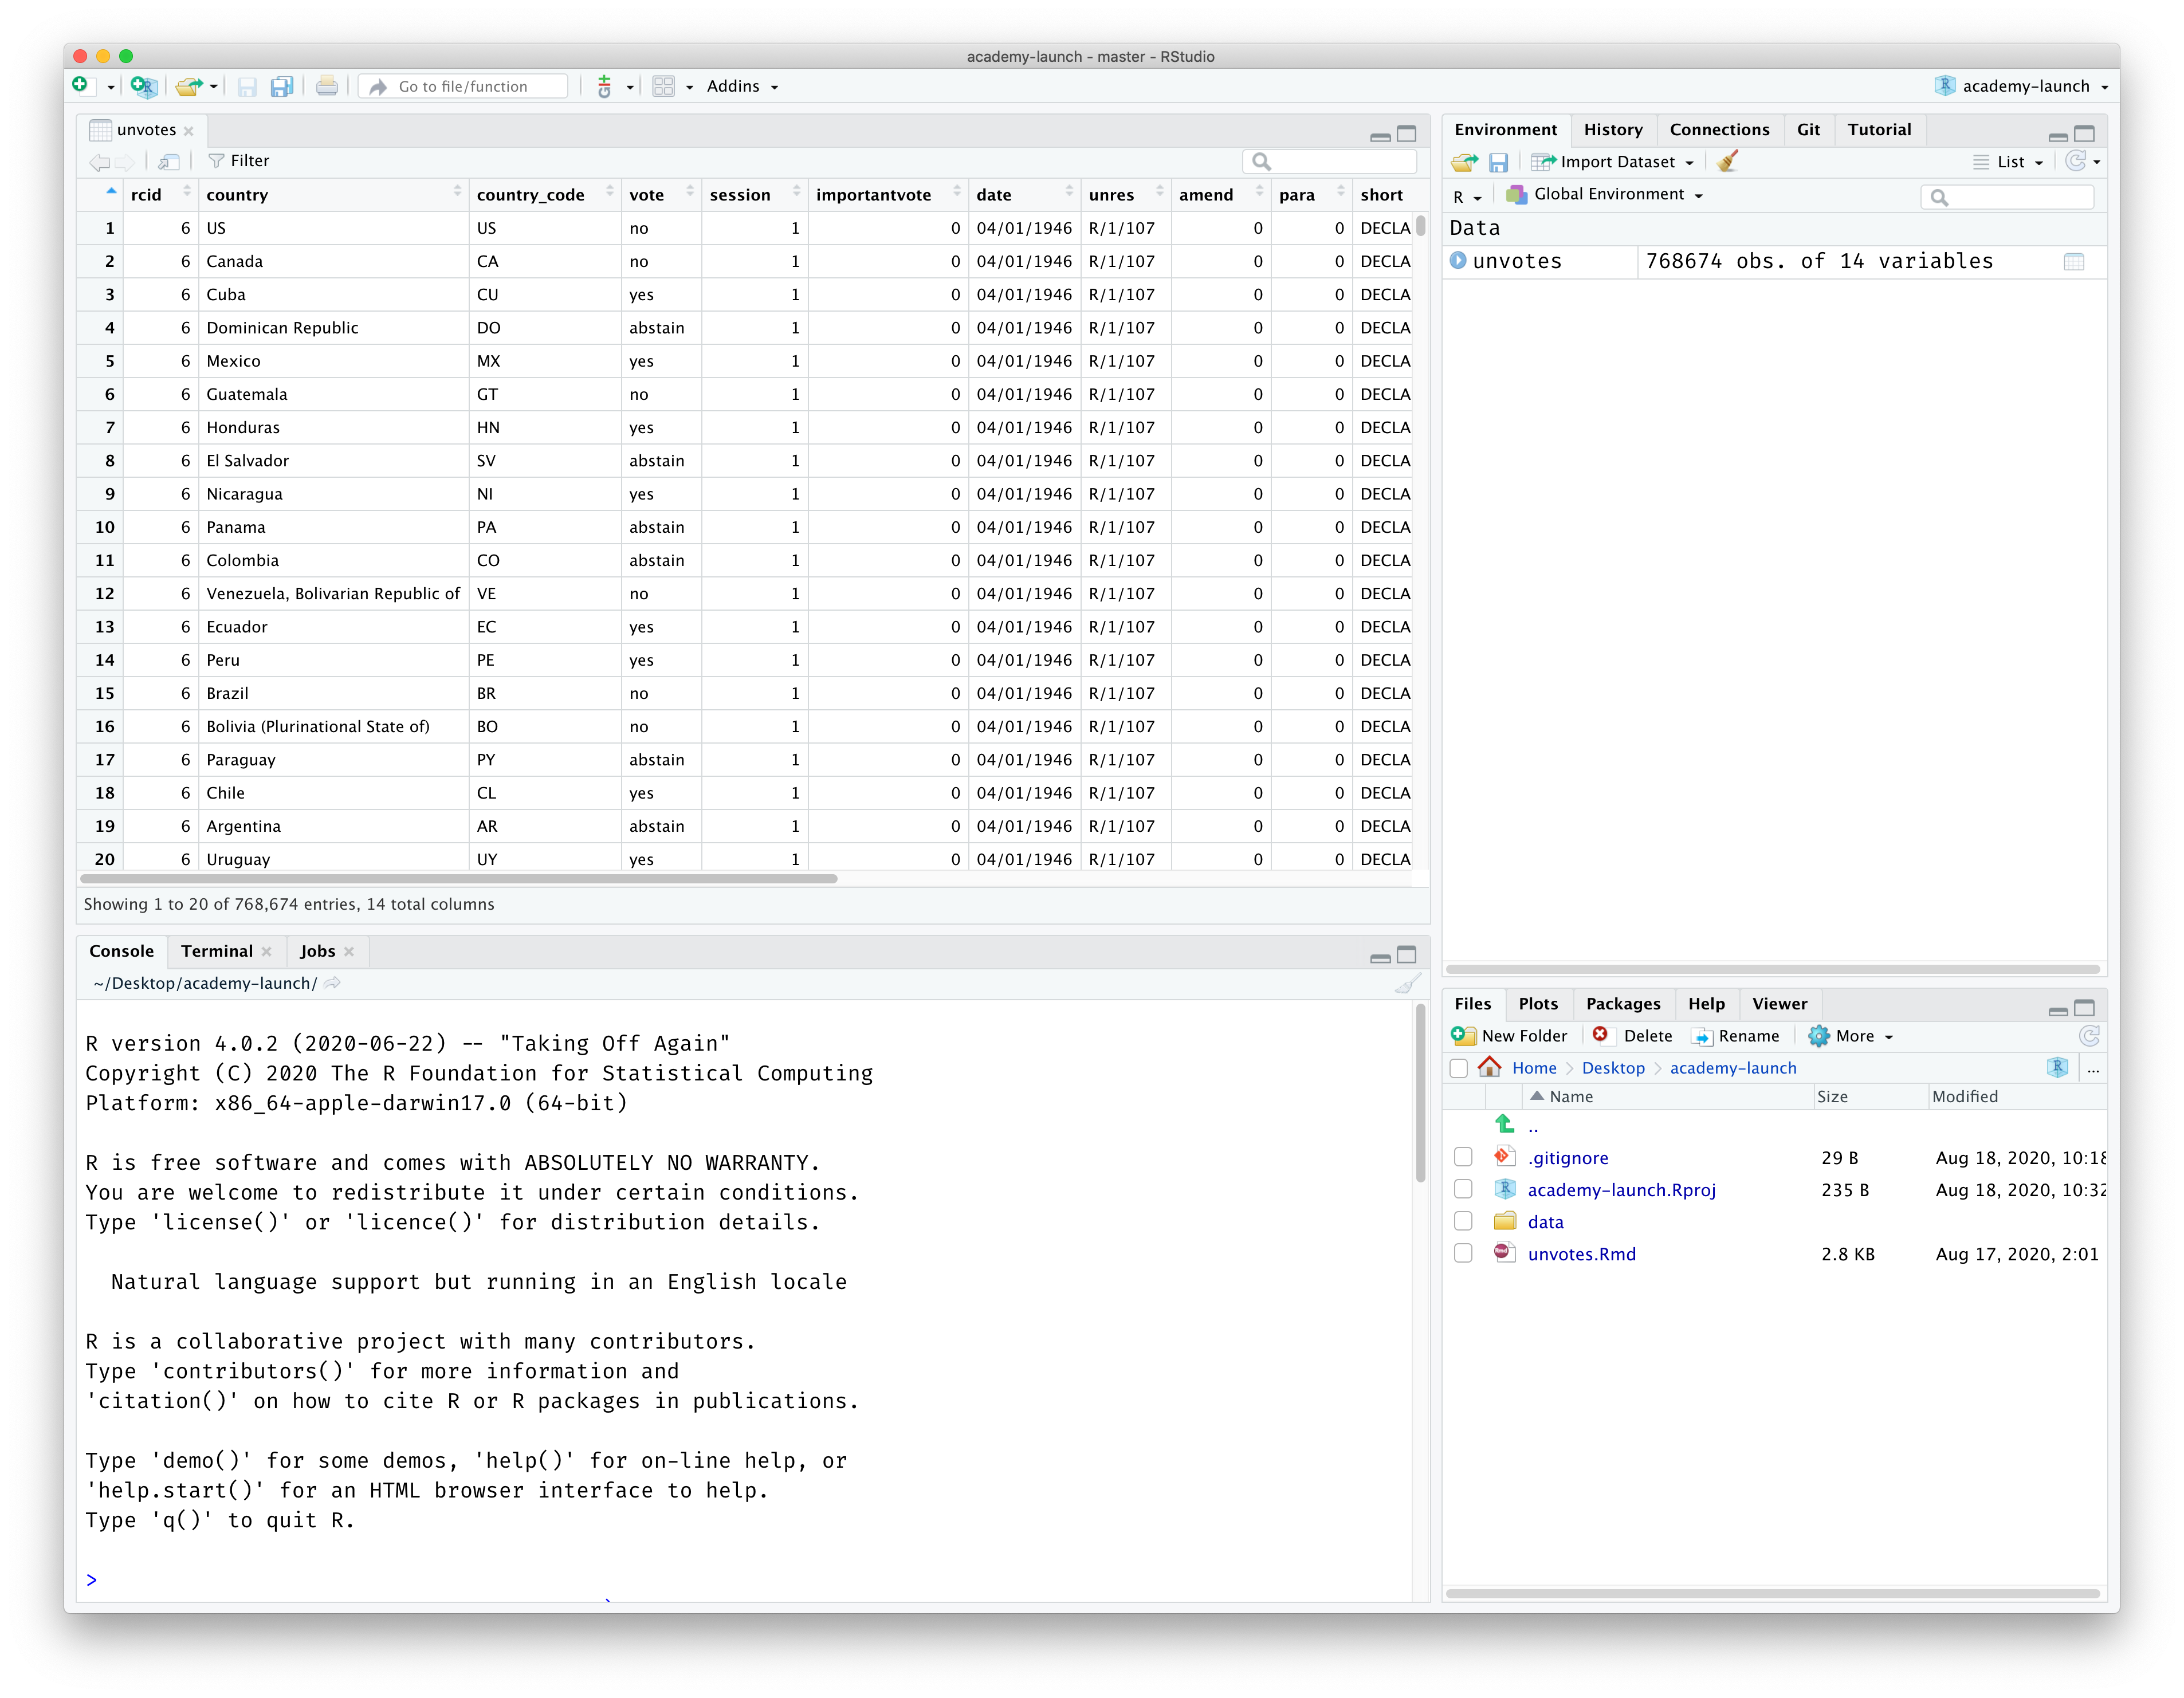
\includegraphics[trim=0cm 0cm 0cm 0cm, clip=true, totalheight=.8\textheight, angle=0]{Images/S1/rstudio}}
			\end{figure}
	\end{frame}
	%------------------------------------------------------------------%
	
	\begin{frame}
		\section{Data \& Empirical Results}
		\frametitle{Data Science Life Cycle}


\begin{figure}
	
	\begin{overprint}
		\onslide<1>\centering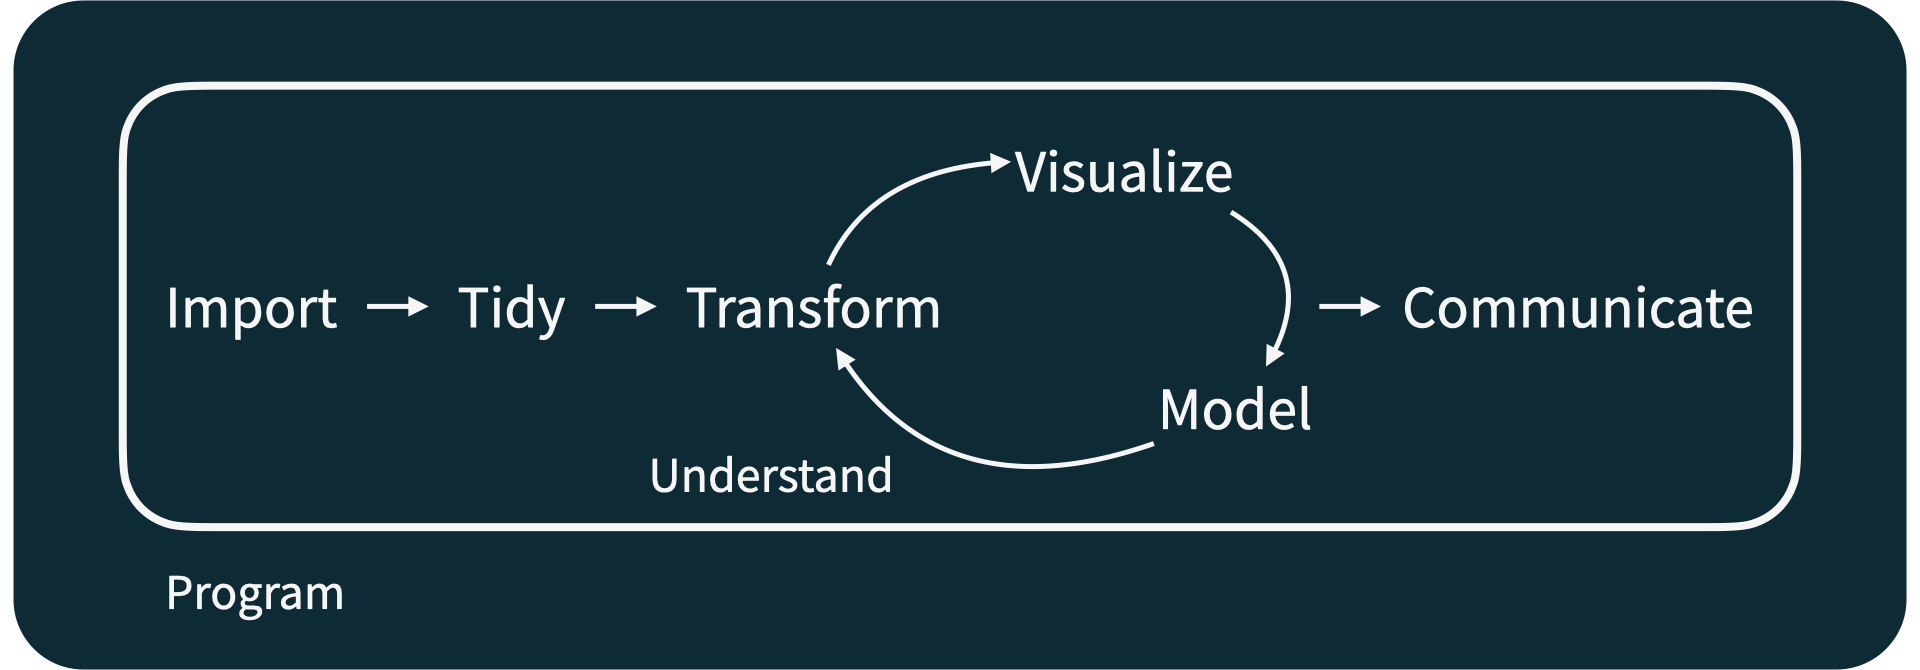
\includegraphics[width=0.8\linewidth]{Images/S1/data-science-cycle/c1}
		\onslide<2>\centering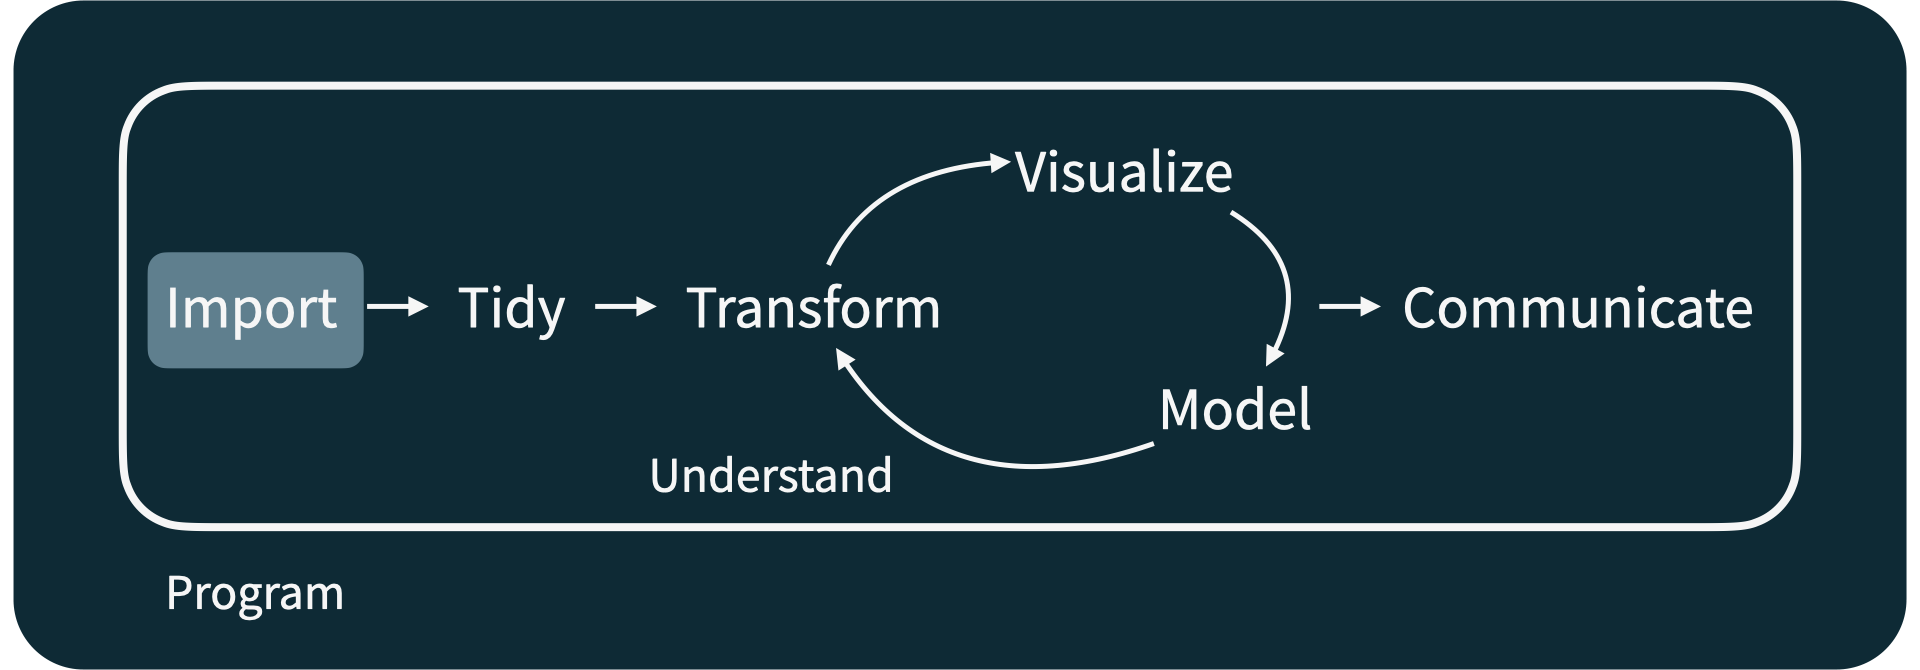
\includegraphics[width=0.8\linewidth]{Images/S1/data-science-cycle/c2}
		\onslide<3>\centering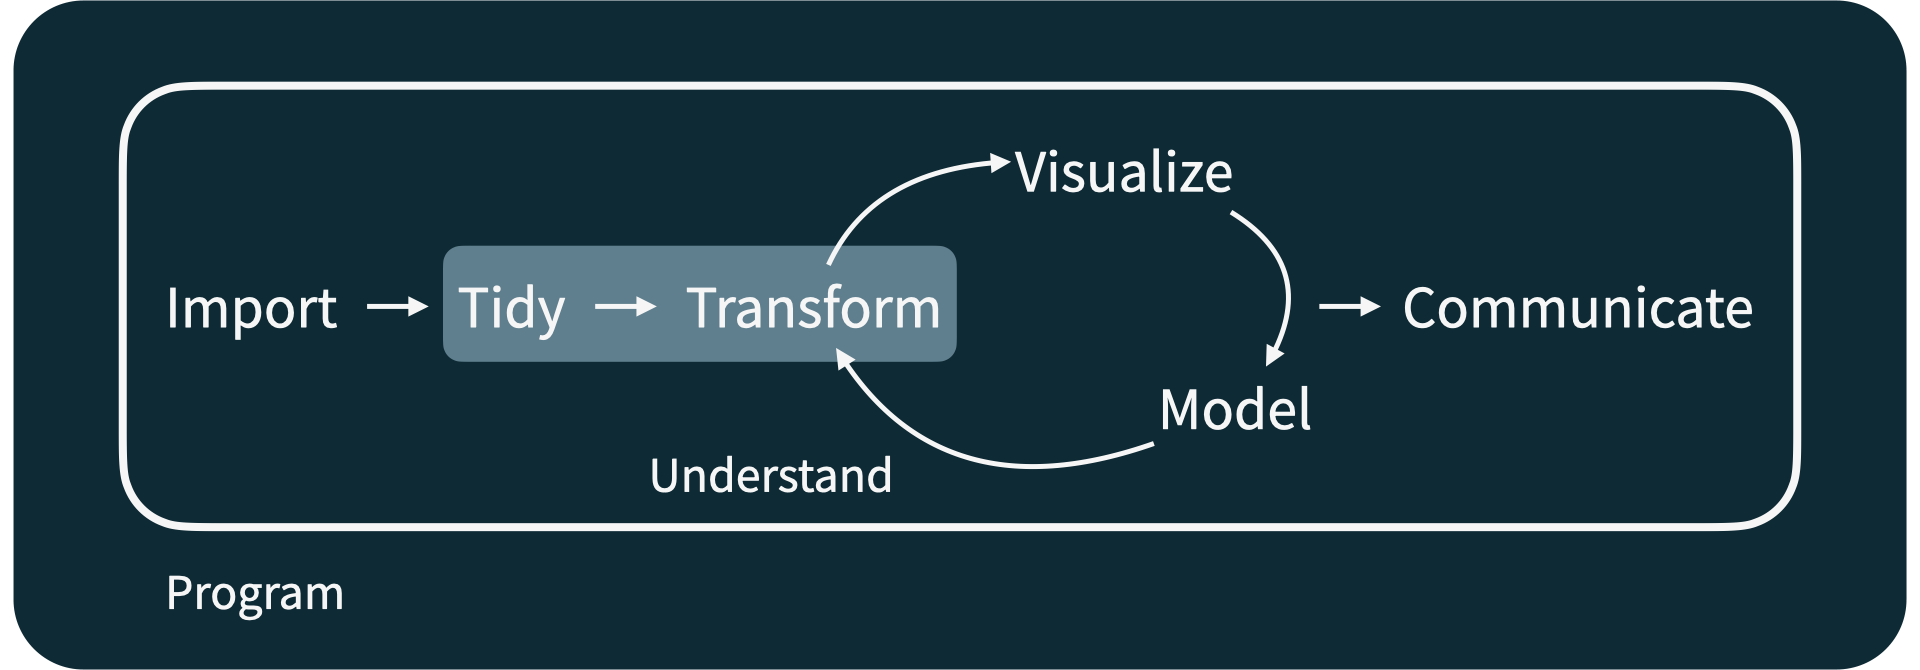
\includegraphics[width=0.8\linewidth]{Images/S1/data-science-cycle/c3}
		\onslide<4>\centering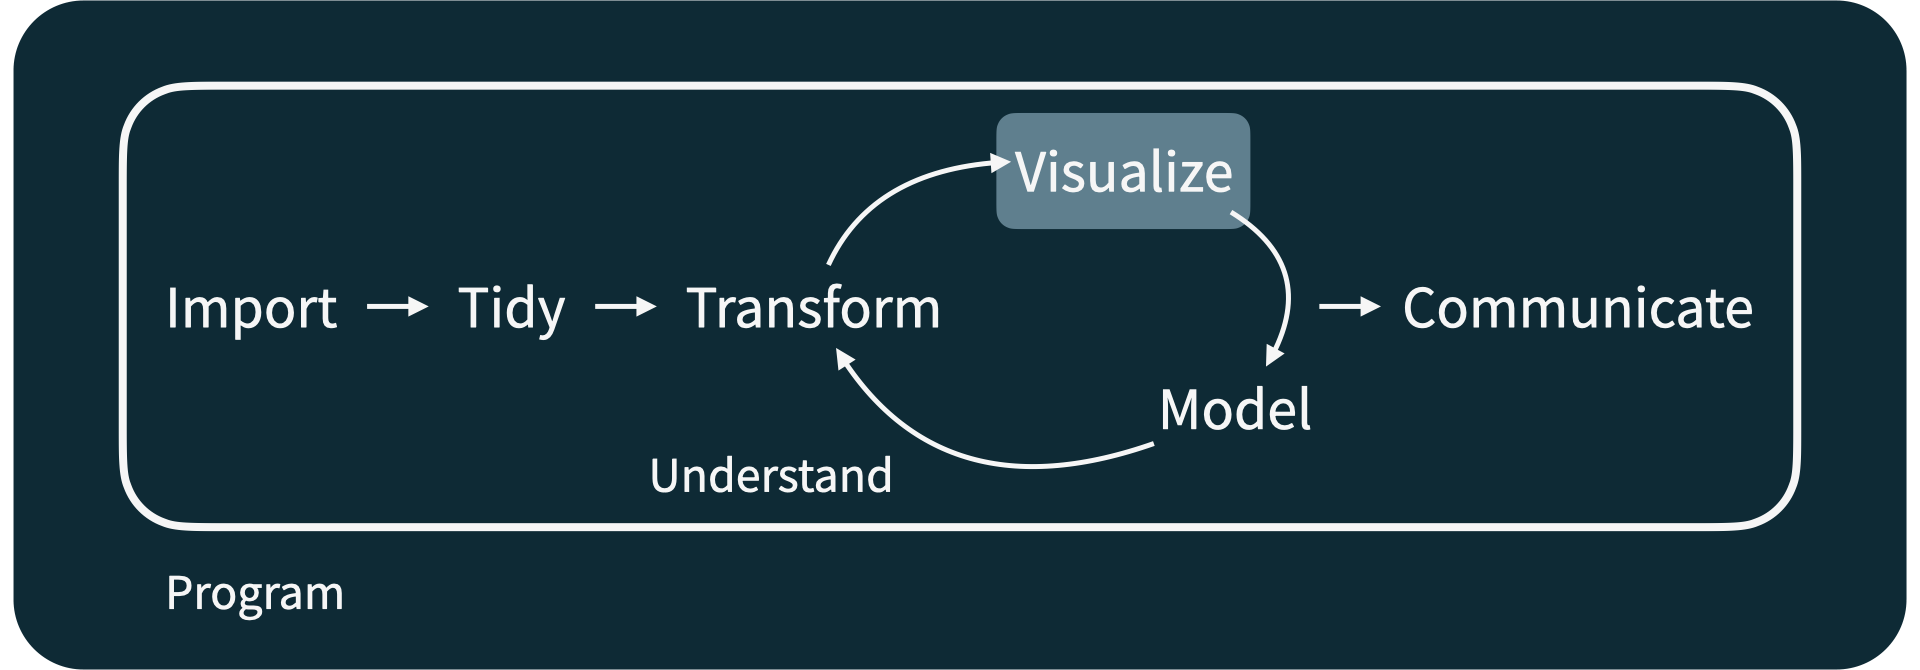
\includegraphics[width=0.8\linewidth]{Images/S1/data-science-cycle/c4}
		\onslide<5>\centering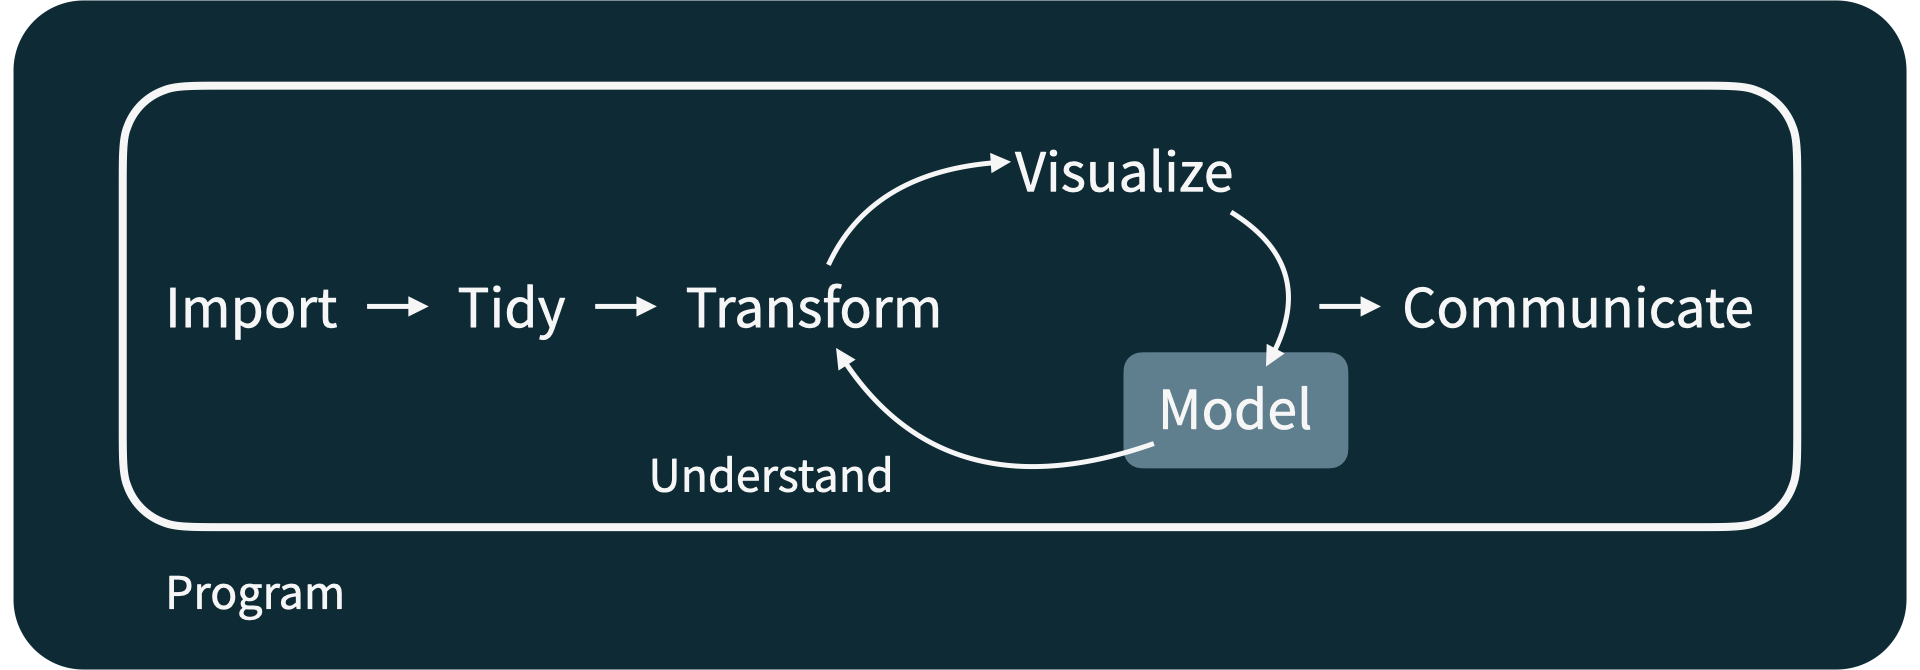
\includegraphics[width=0.8\linewidth]{Images/S1/data-science-cycle/c5}
		\onslide<6>\centering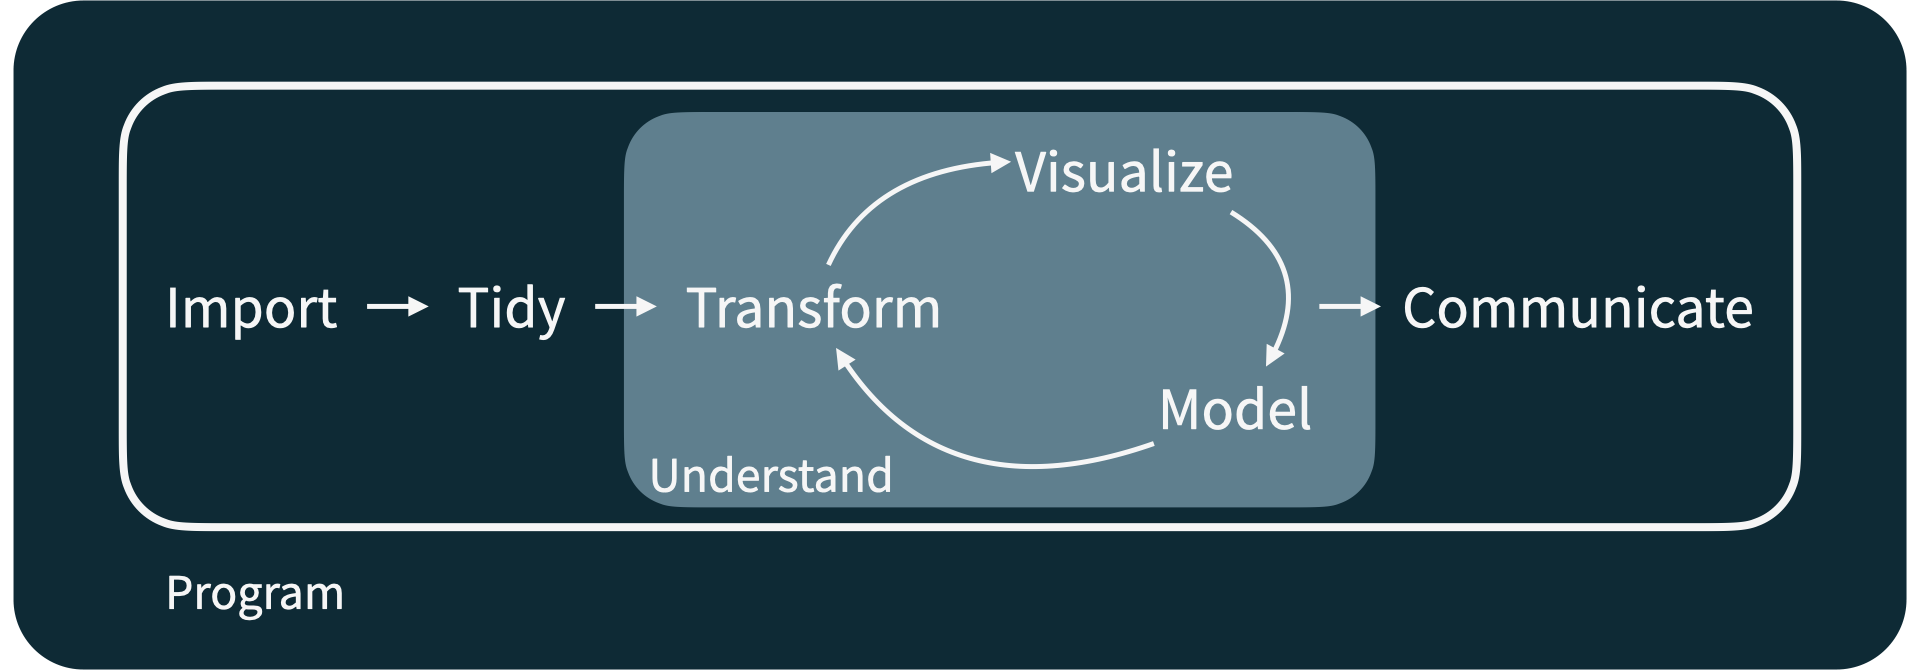
\includegraphics[width=0.8\linewidth]{Images/S1/data-science-cycle/c6}
		\onslide<7>\centering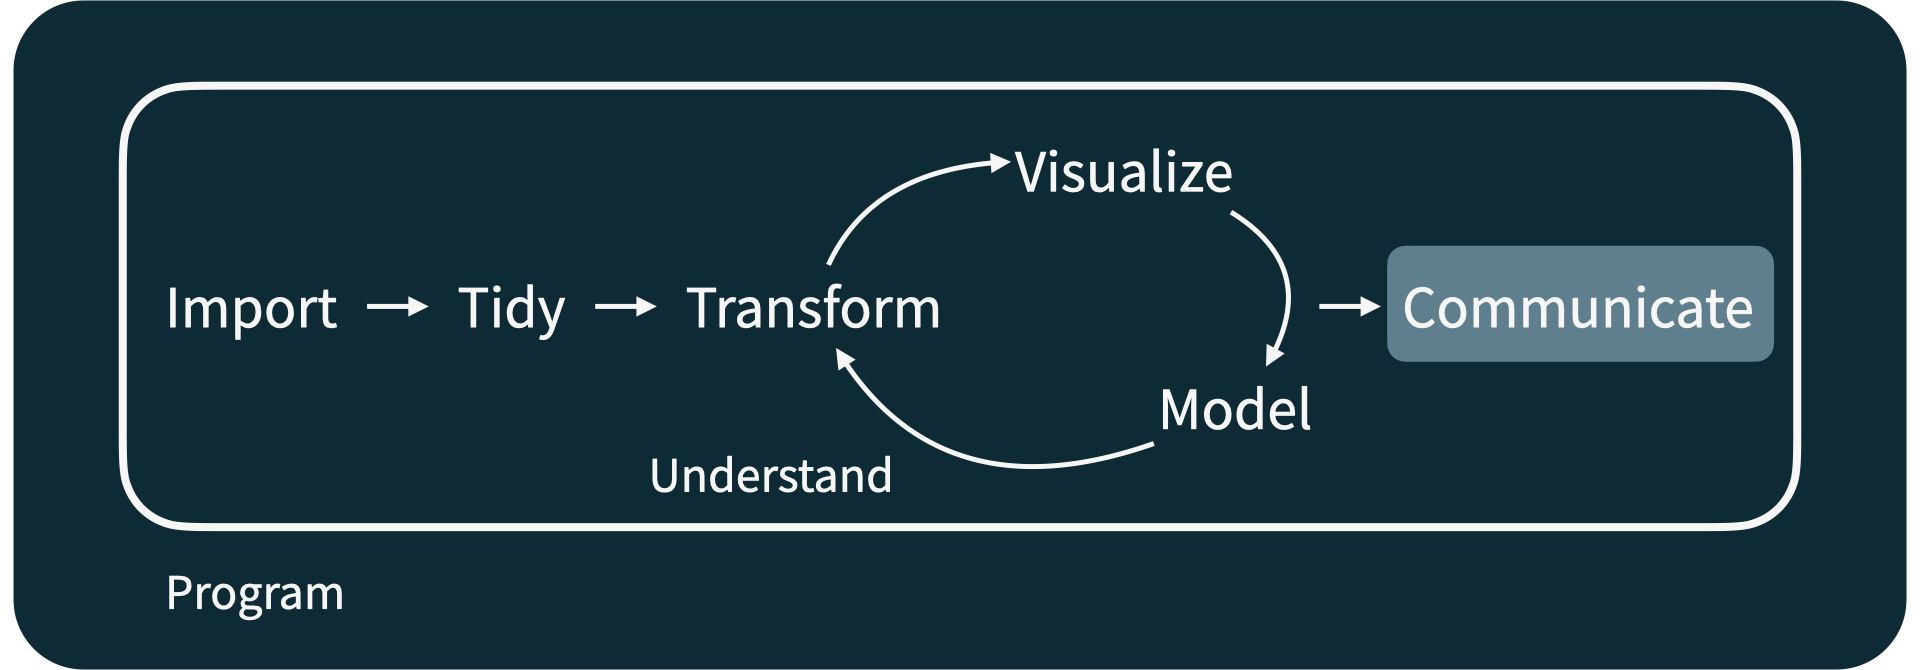
\includegraphics[width=0.8\linewidth]{Images/S1/data-science-cycle/c7}
		\onslide<8>\centering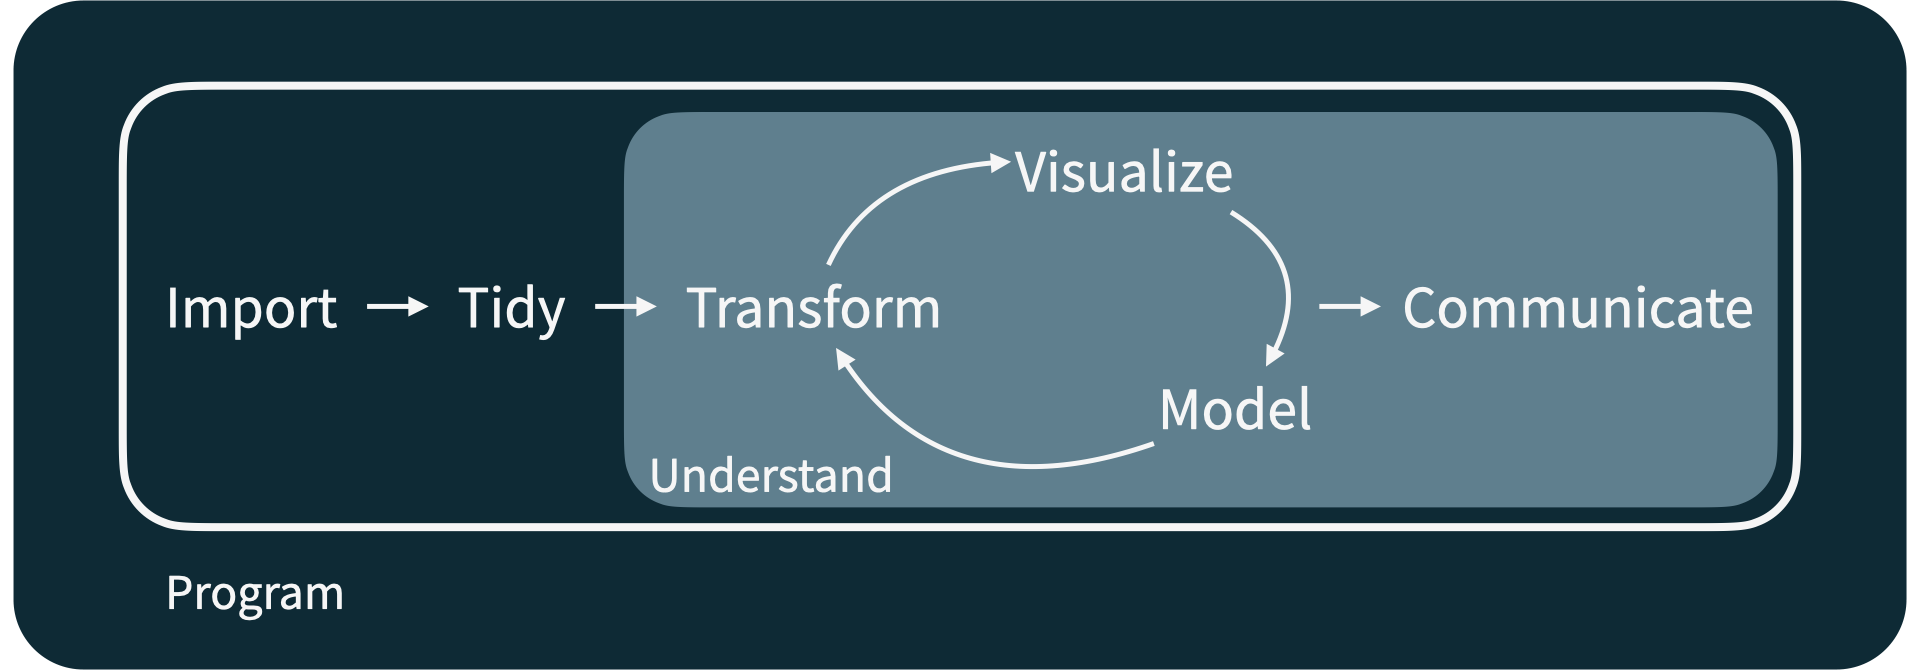
\includegraphics[width=0.8\linewidth]{Images/S1/data-science-cycle/c8}
		\onslide<9>\centering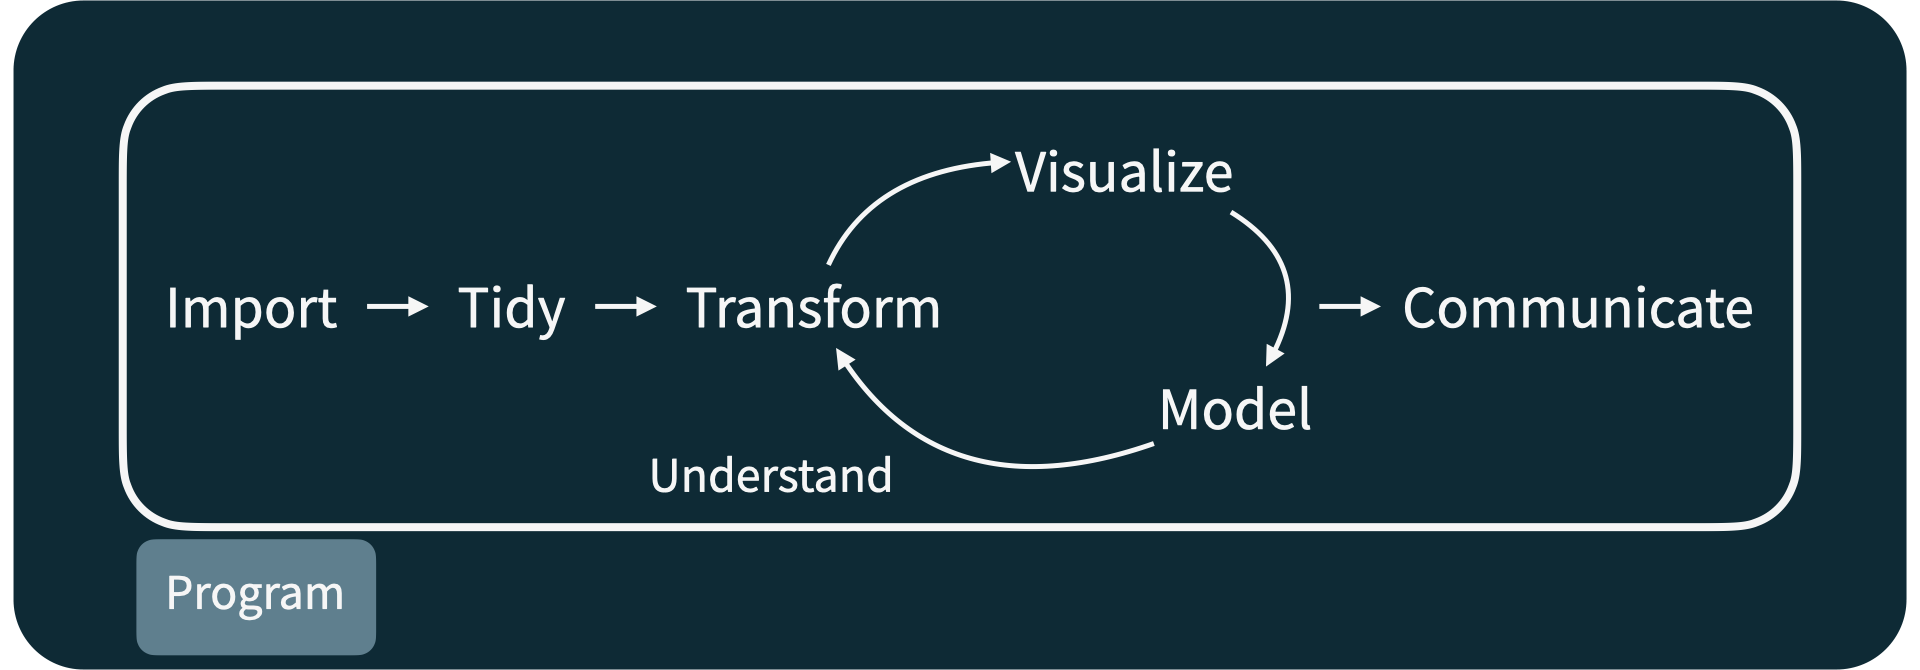
\includegraphics[width=0.8\linewidth]{Images/S1/data-science-cycle/c9}	
		
	\end{overprint}
\end{figure}
		
	\end{frame}
	%------------------------------------------------------------------%
	
	
		%------------------------------------------------------------------%





		\section{Conclusions}

\begin{frame}
	

\begin{figure}
	
	\begin{overprint}
		\onslide<1>\centering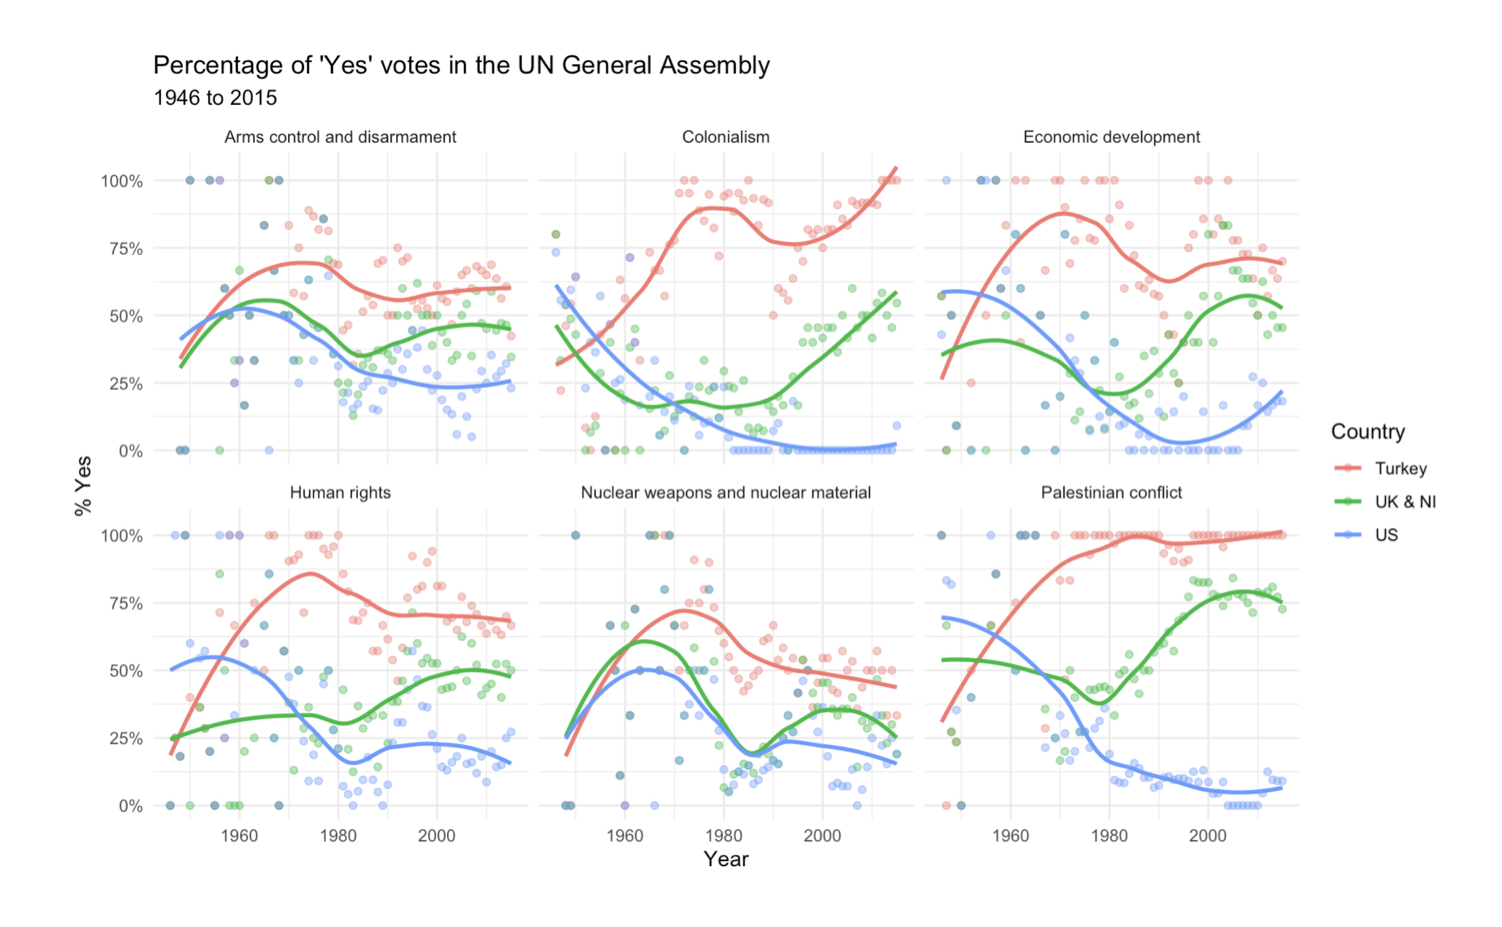
\includegraphics[width=.9\linewidth]{Images/S1/unvotes/unvotes-01}
		\onslide<2>\centering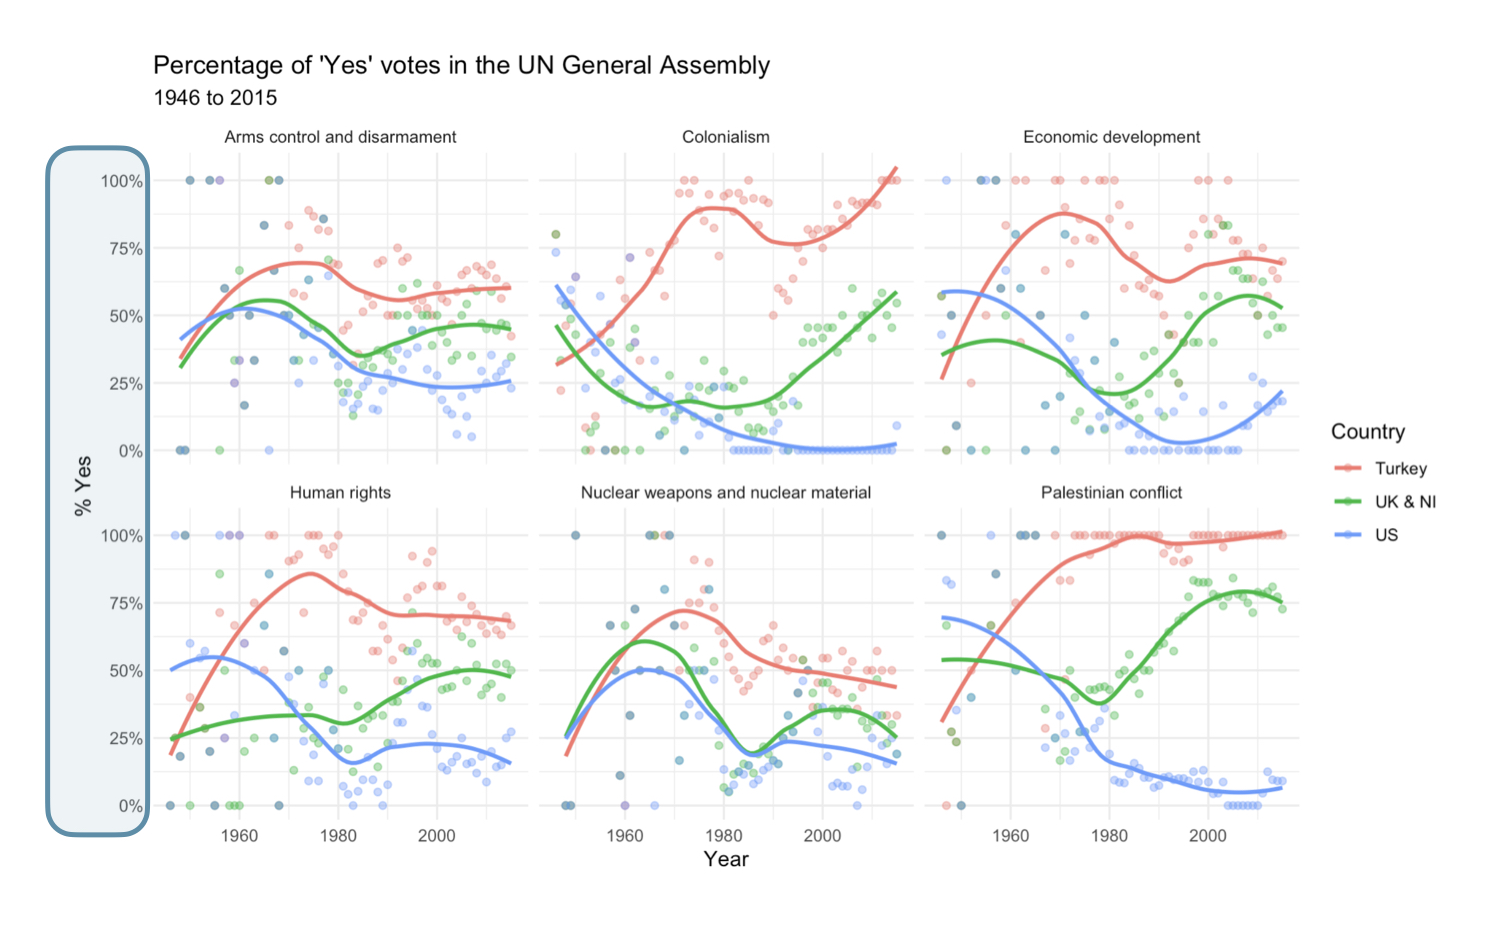
\includegraphics[width=0.9\linewidth]{Images/S1/unvotes/unvotes-02}
		\onslide<3>\centering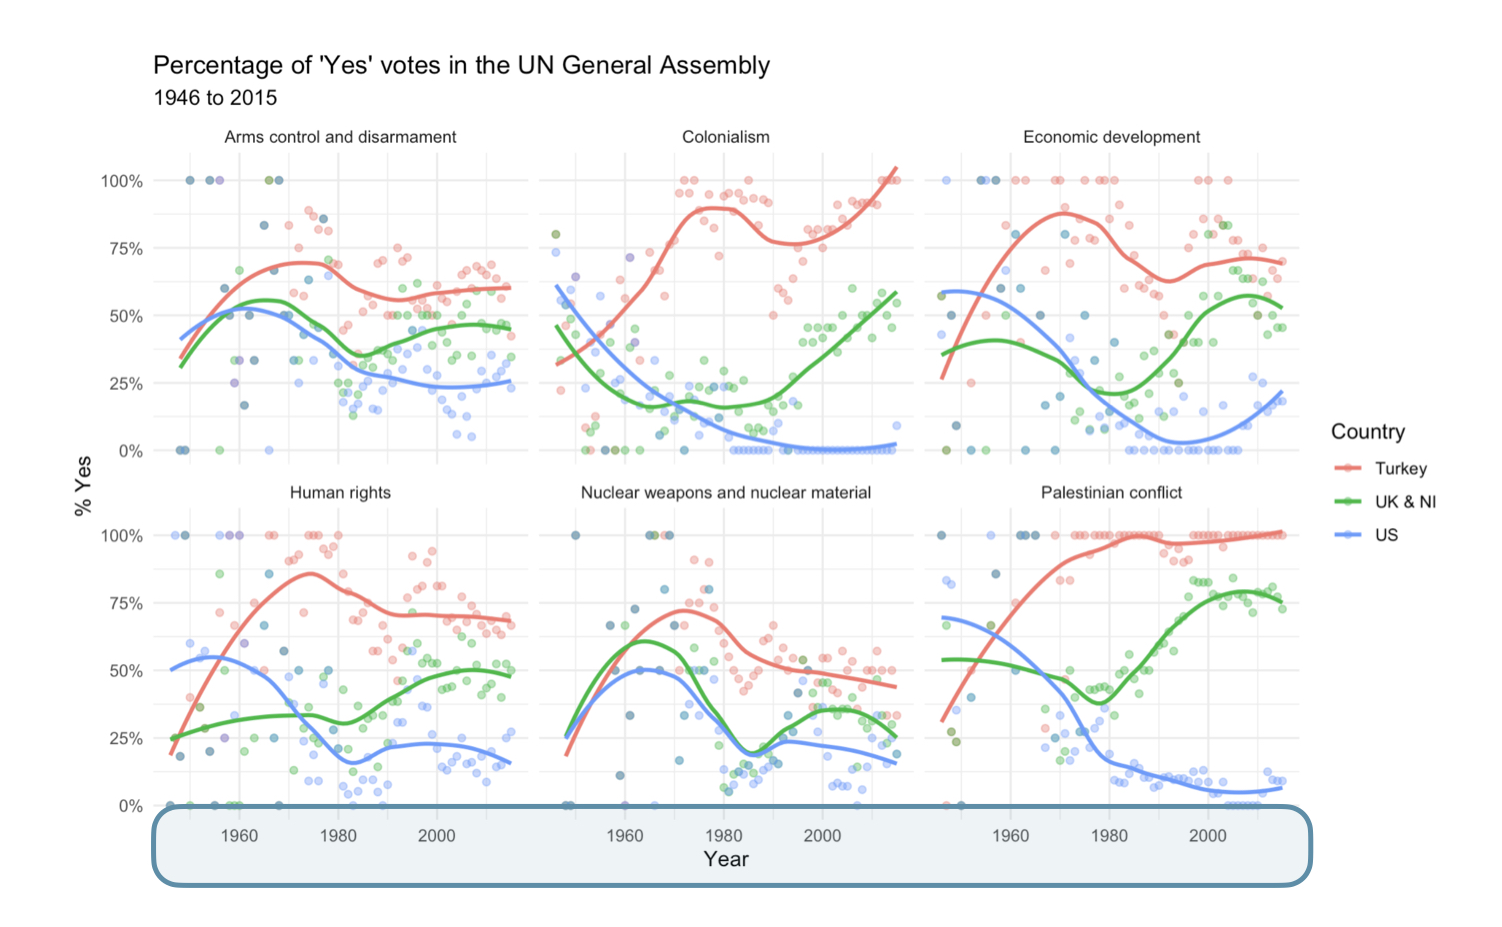
\includegraphics[width=0.9\linewidth]{Images/S1/unvotes/unvotes-03}
		\onslide<4>\centering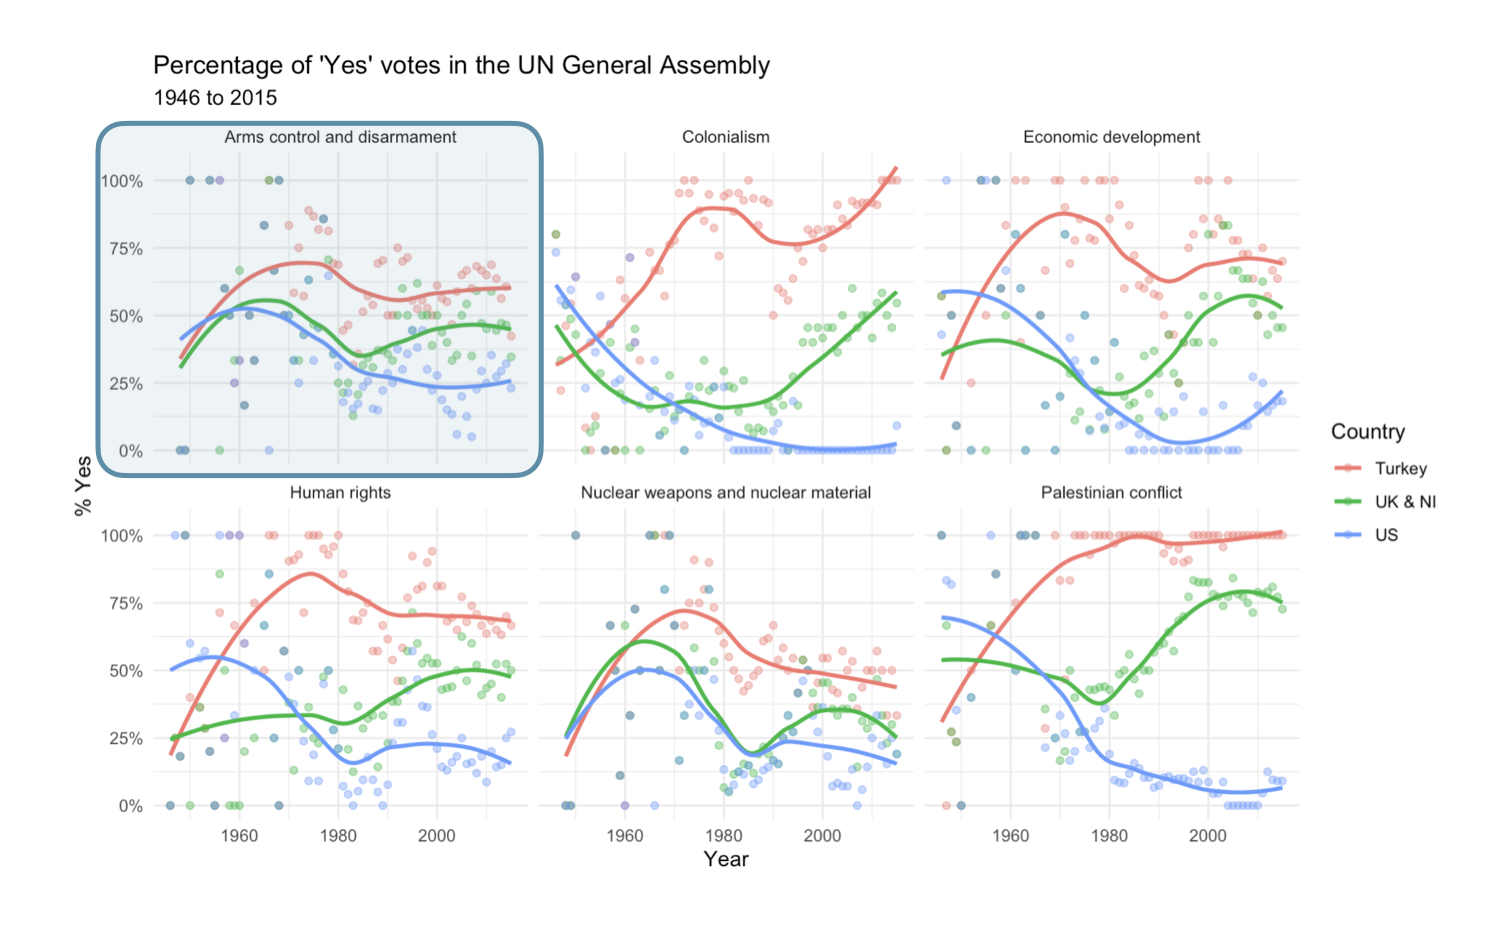
\includegraphics[width=0.9\linewidth]{Images/S1/unvotes/unvotes-04}
		\onslide<5>\centering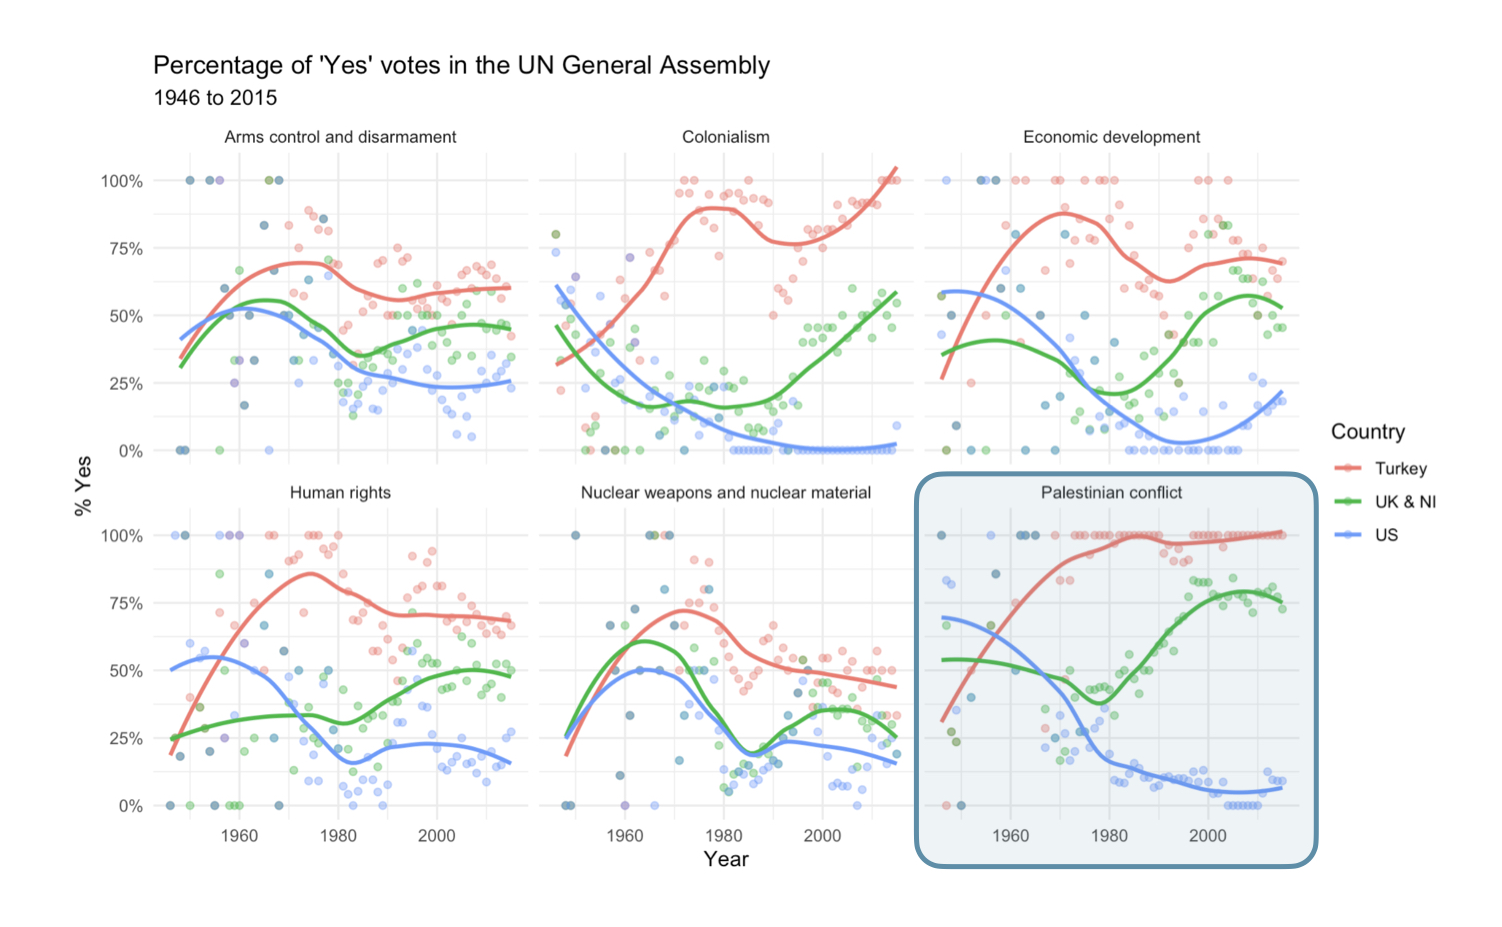
\includegraphics[width=0.9\linewidth]{Images/S1/unvotes/unvotes-05}	
	\end{overprint}
\end{figure}

\end{frame}

	%------------------------------------------------------------------%
	
	\begin{frame}
	\begin{figure}
		\centering
		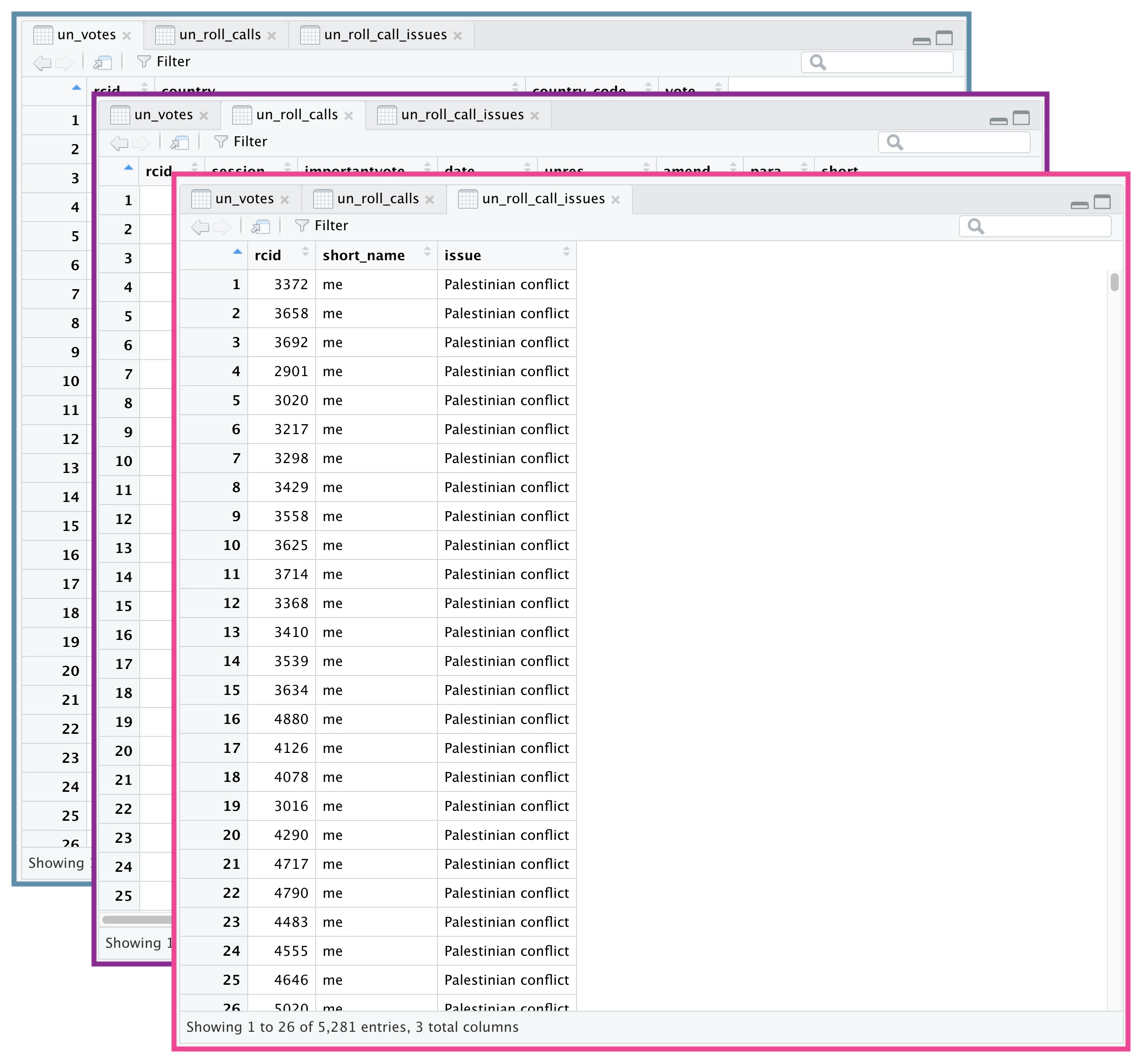
\includegraphics[width=0.5\linewidth]{Images/S1/unvotes/unvotes-07}
		\label{fig:unvotes-07}
	\end{figure}
	
	\end{frame}
	%------------------------------------------------------------------%
	
	\begin{frame}
		\begin{figure}
			\vspace{1em}
			\begin{overprint}
				\onslide<1>\centering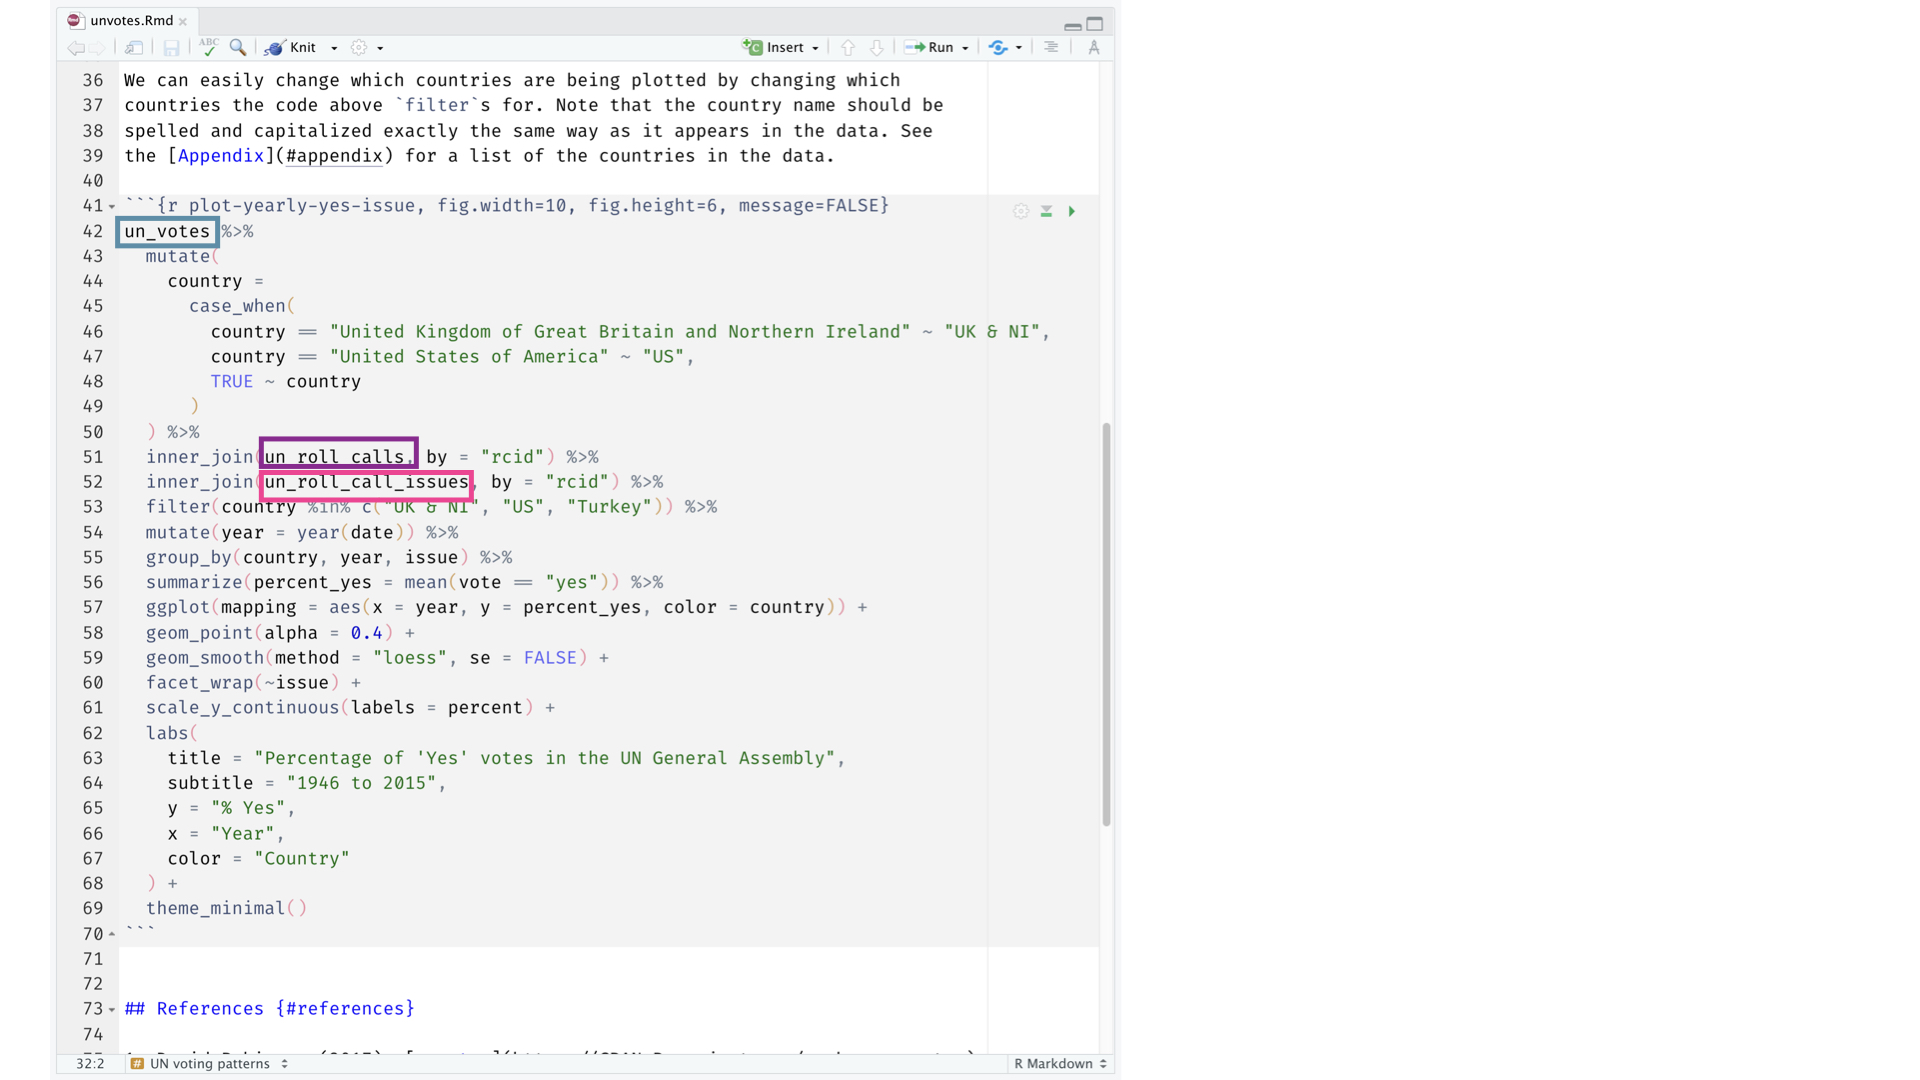
\includegraphics[width=.9\linewidth]{Images/S1/unvotes/unvotes-08}
				\onslide<2>\centering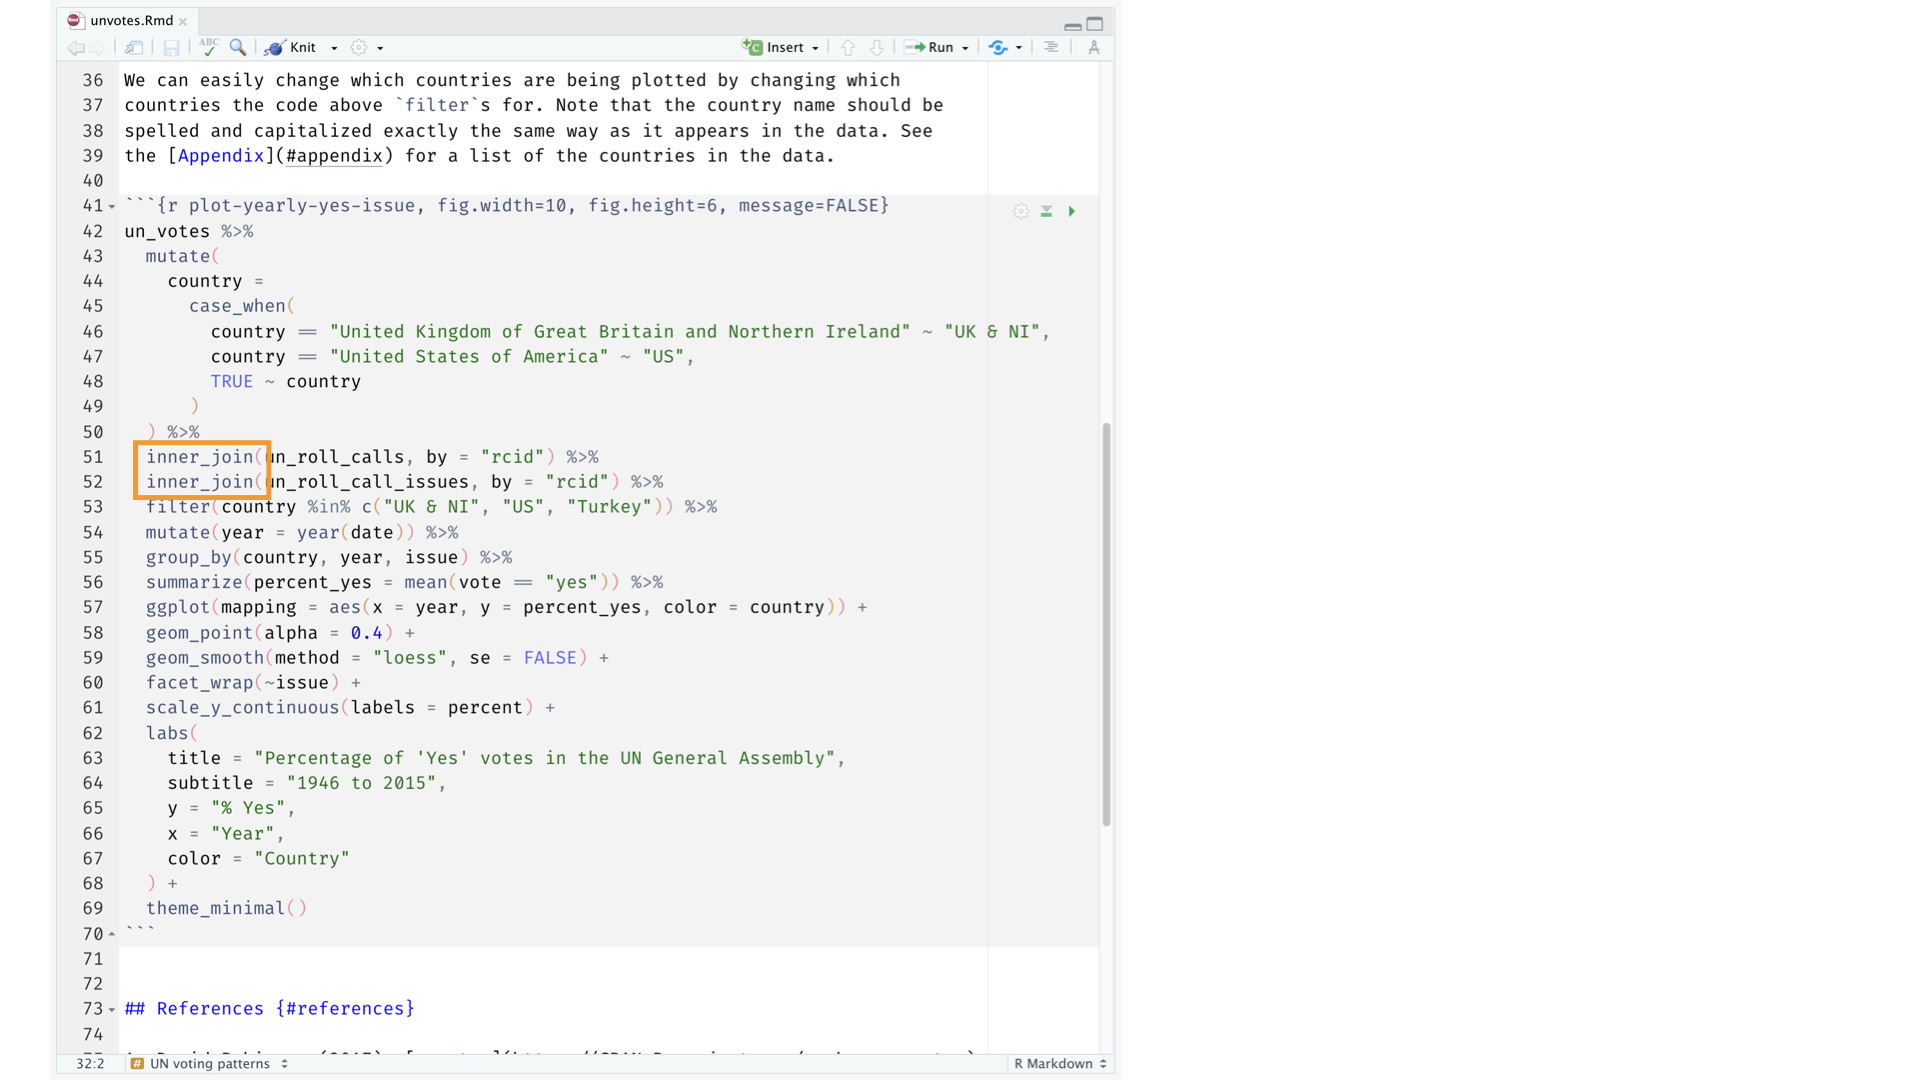
\includegraphics[width=0.9\linewidth]{Images/S1/unvotes/unvotes-09}
				\onslide<3>\centering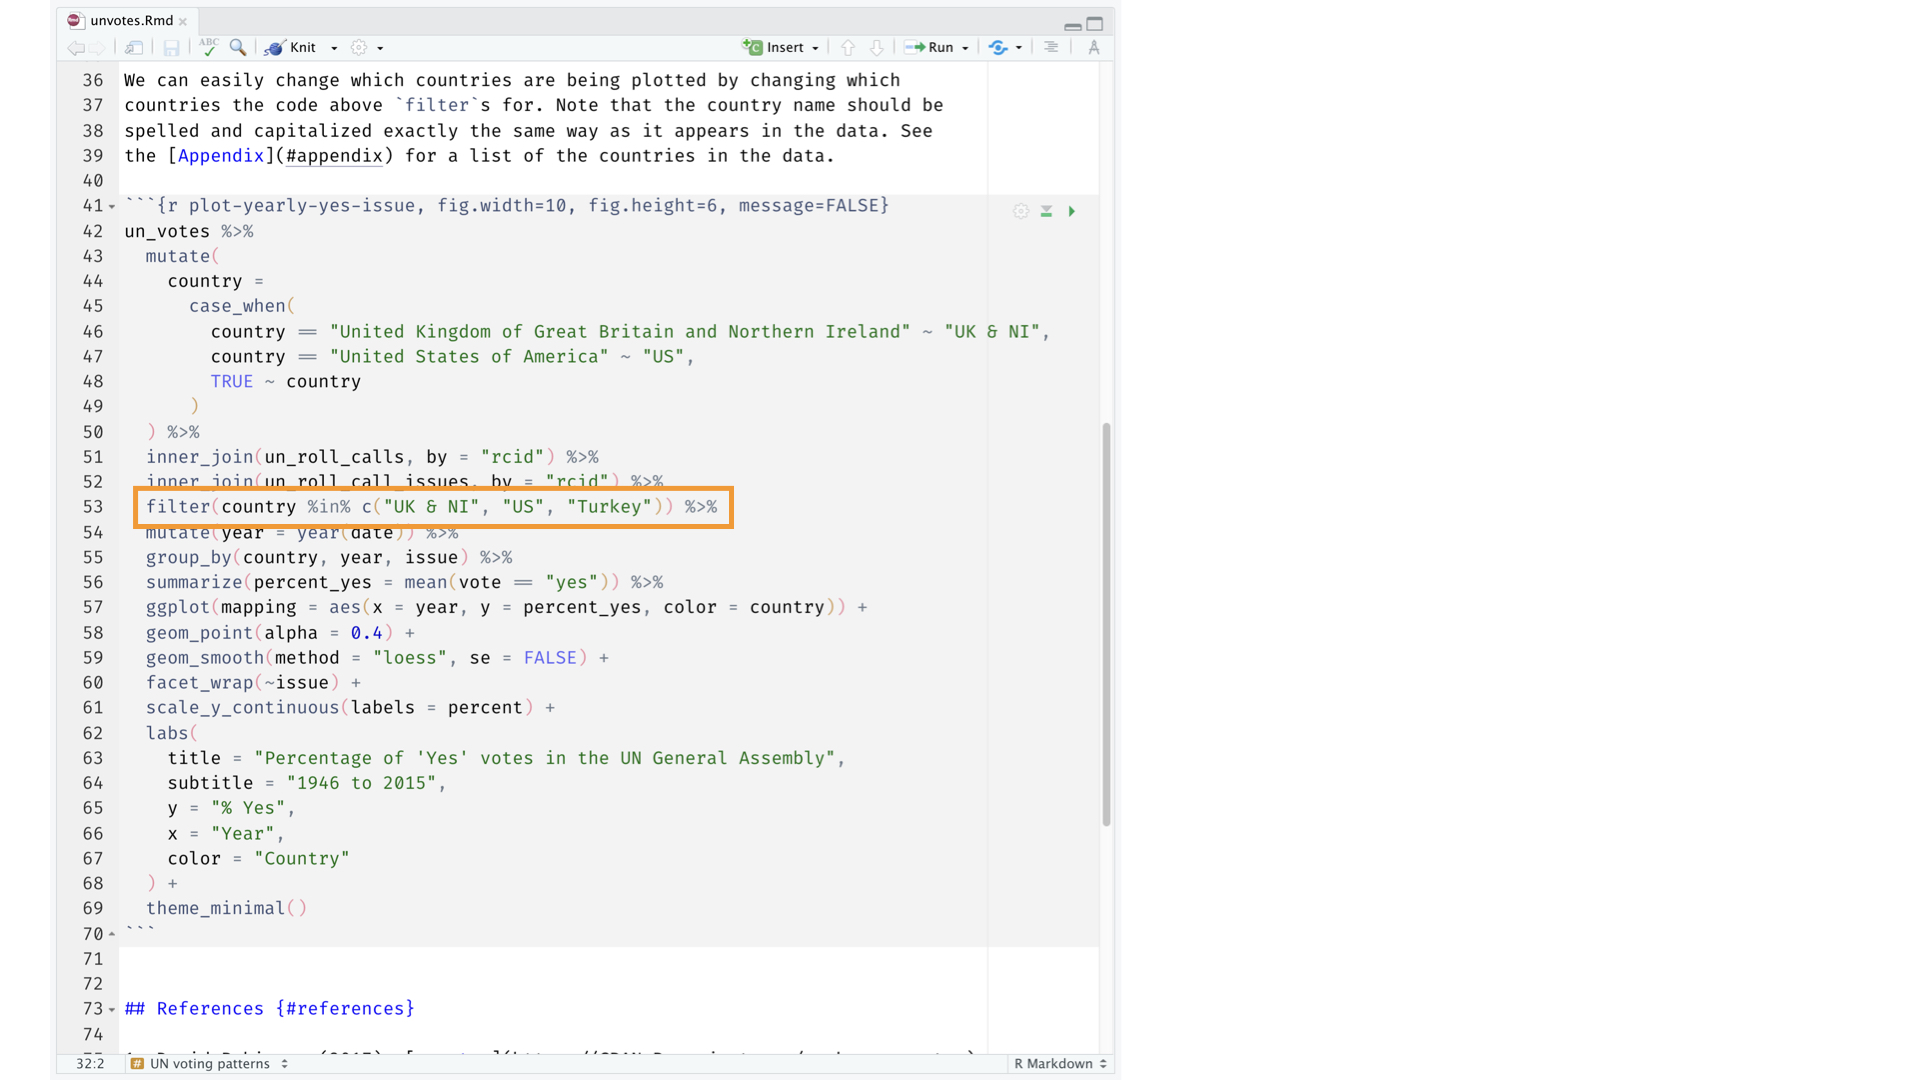
\includegraphics[width=0.9\linewidth]{Images/S1/unvotes/unvotes-10}
				\onslide<4>\centering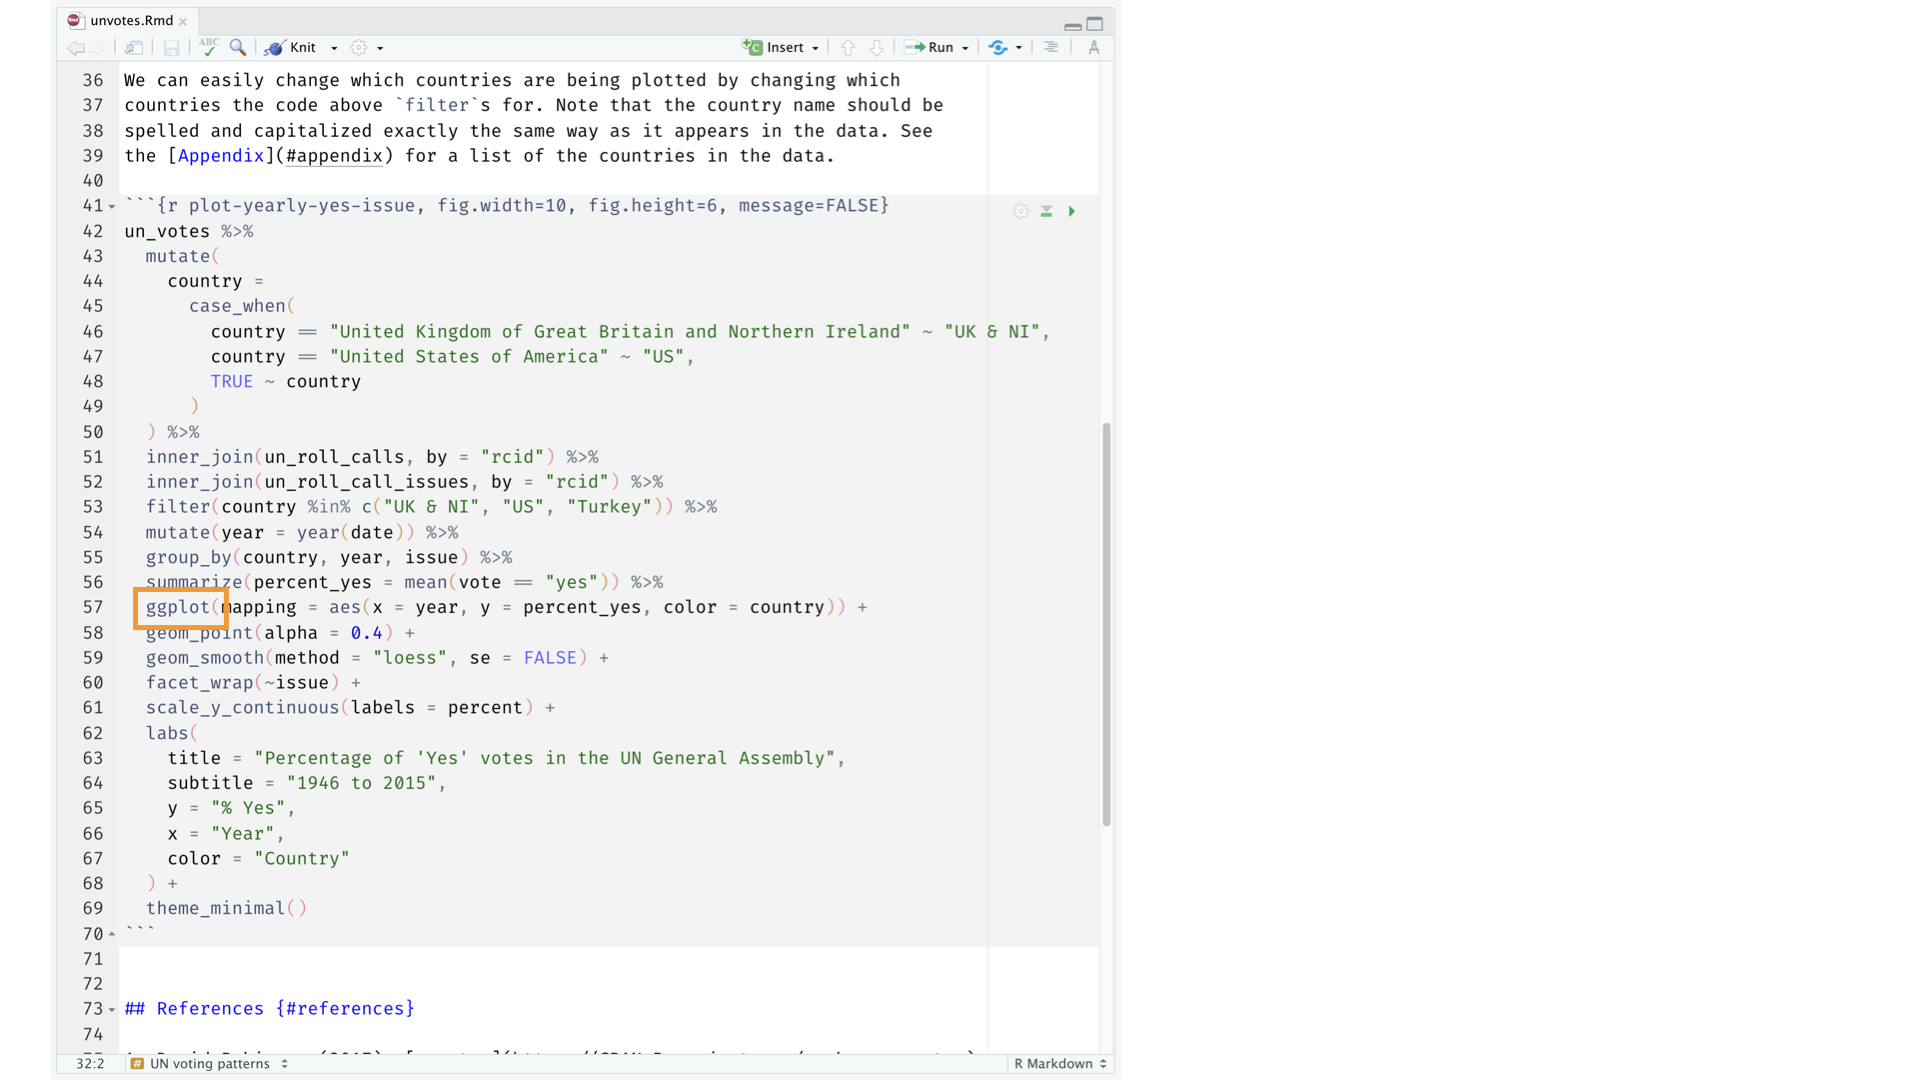
\includegraphics[width=0.9\linewidth]{Images/S1/unvotes/unvotes-11}
				\onslide<5>\centering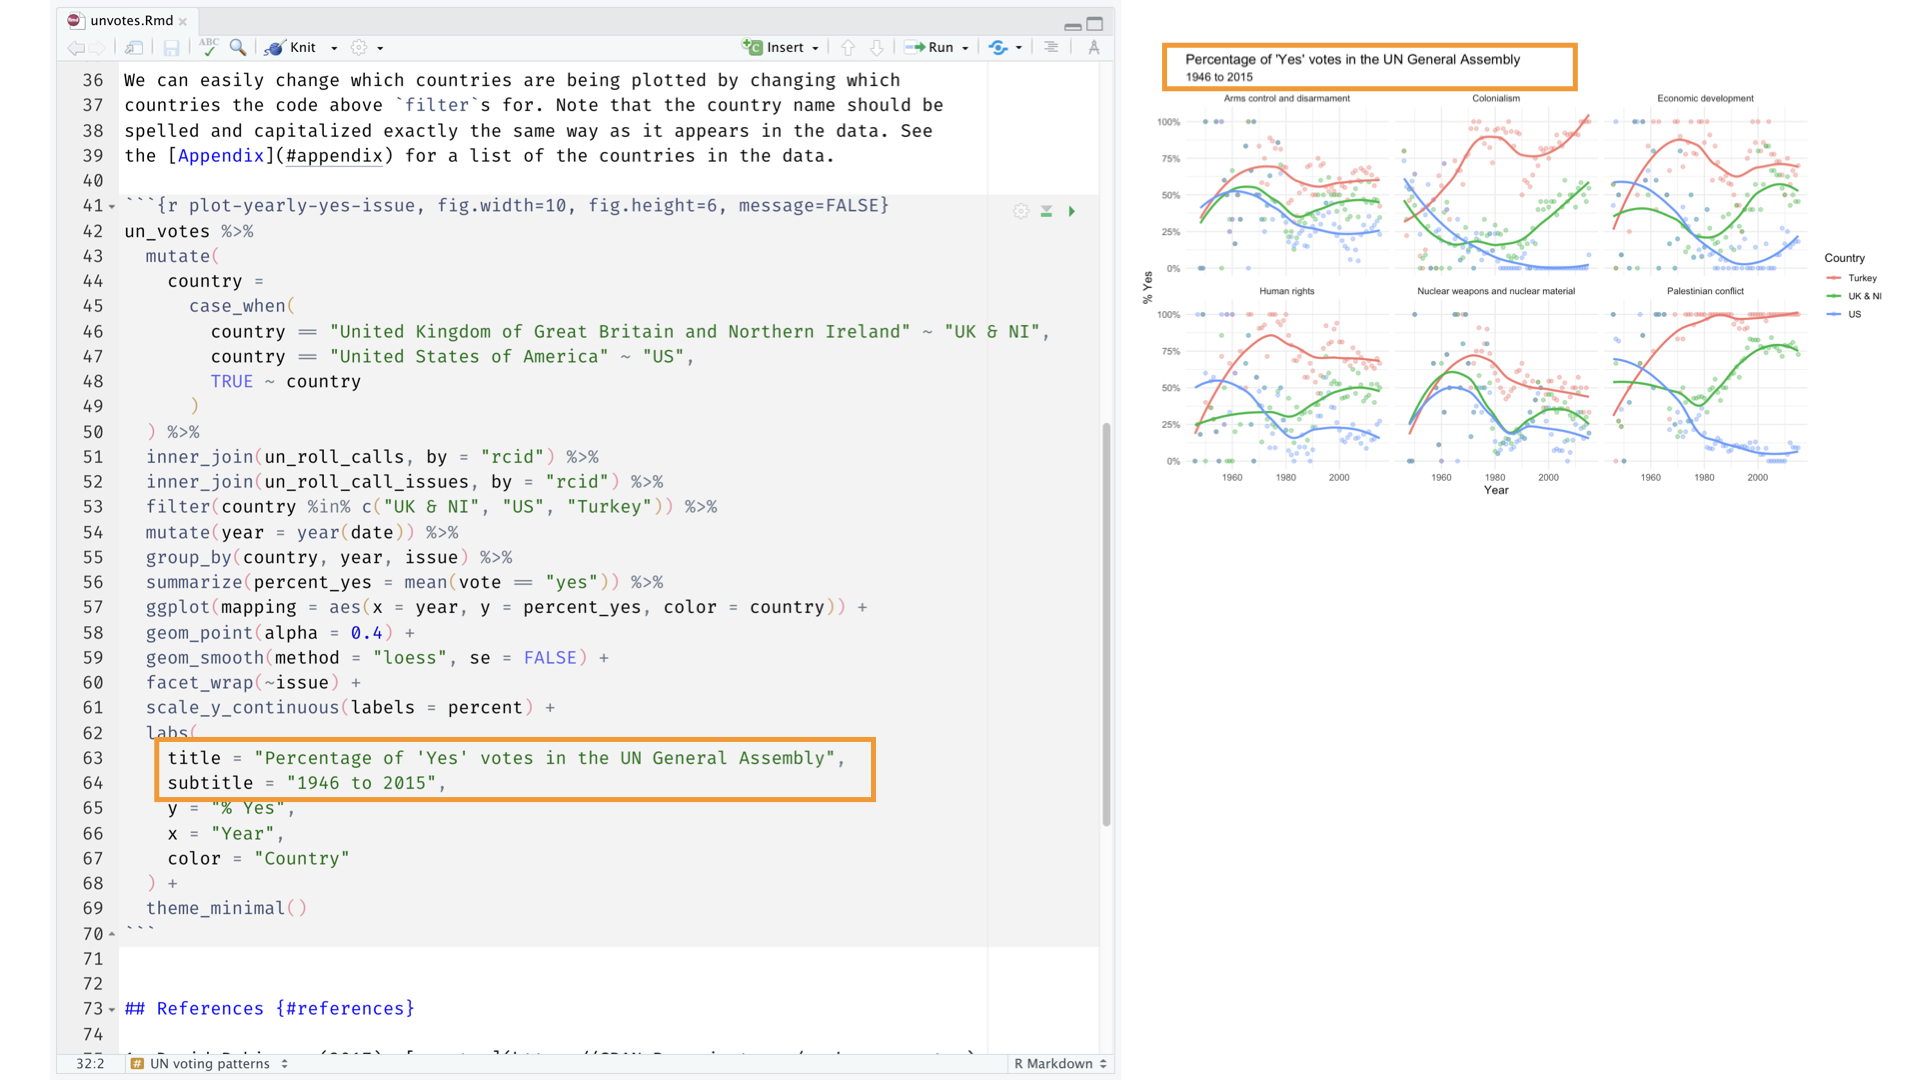
\includegraphics[width=0.9\linewidth]{Images/S1/unvotes/unvotes-12}	
				\onslide<6>\centering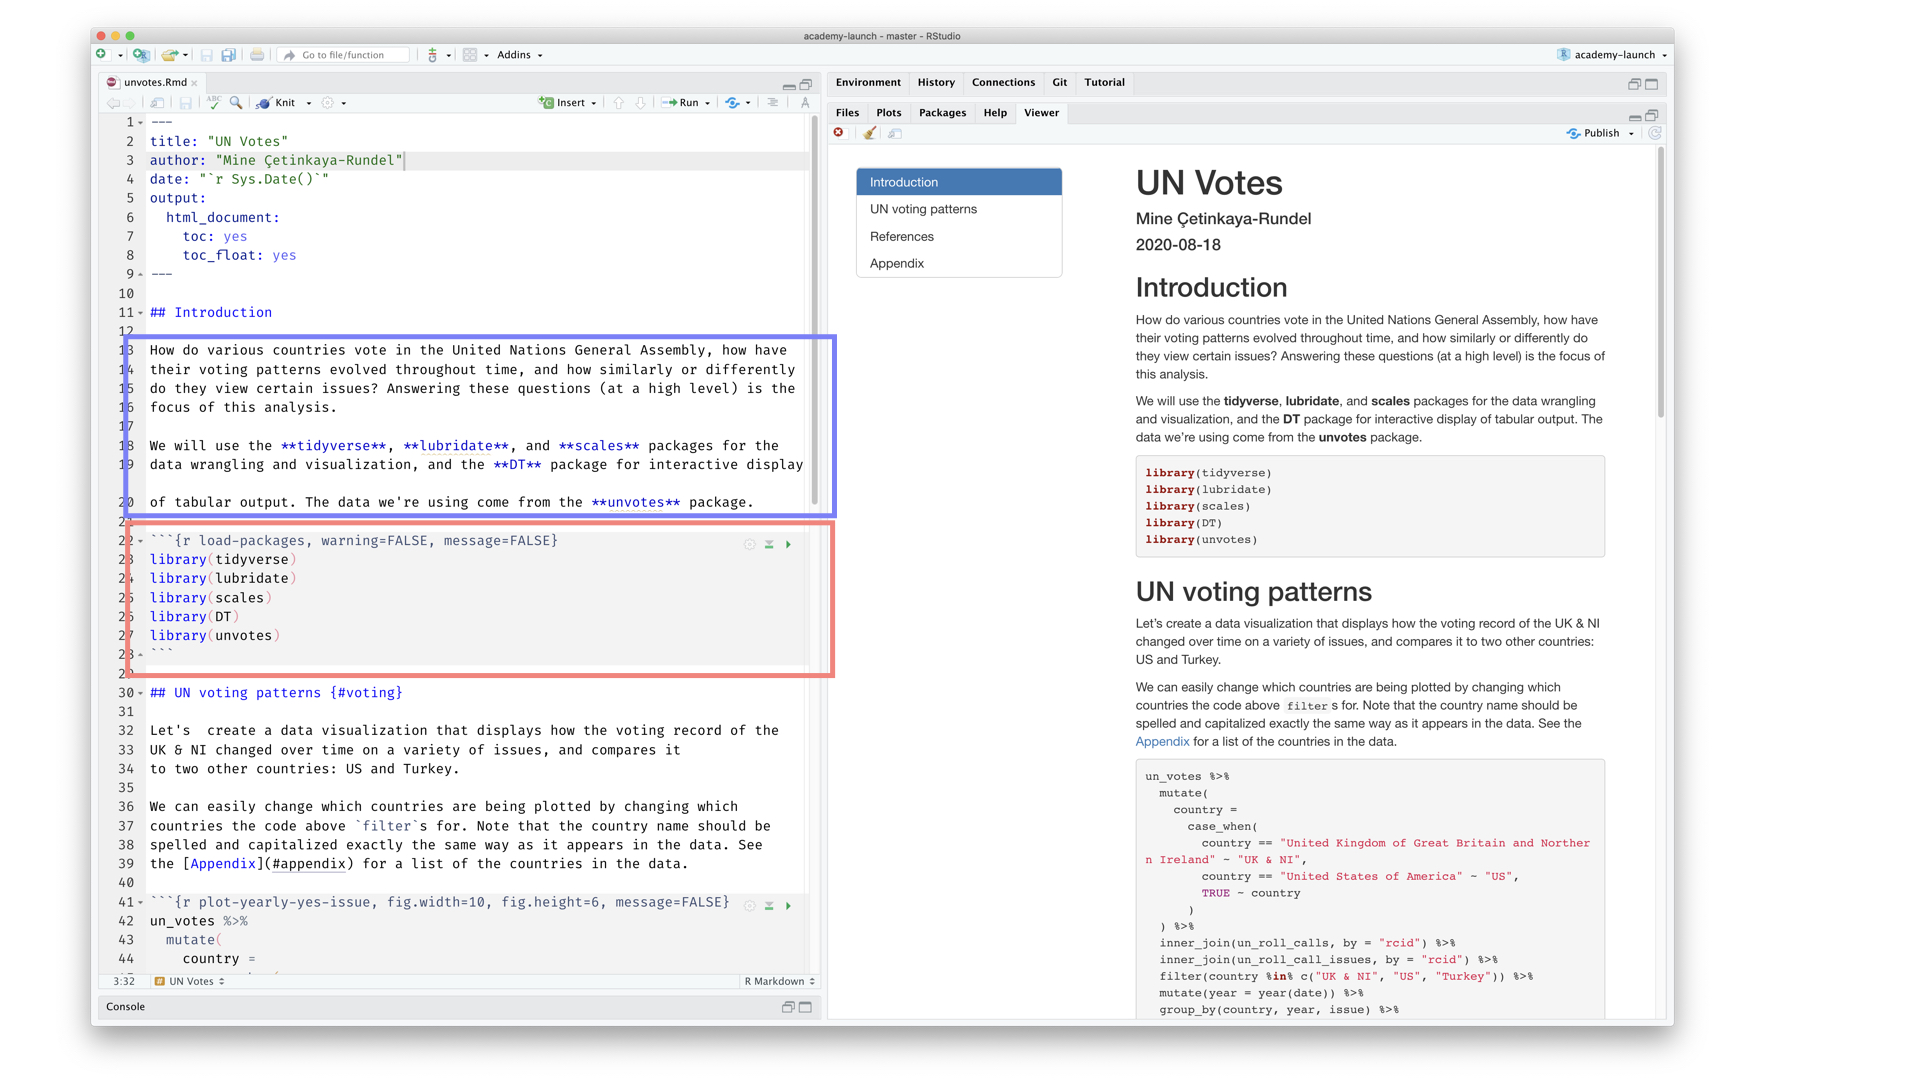
\includegraphics[width=0.9\linewidth]{Images/S1/unvotes/unvotes-13}	
				\onslide<7>\centering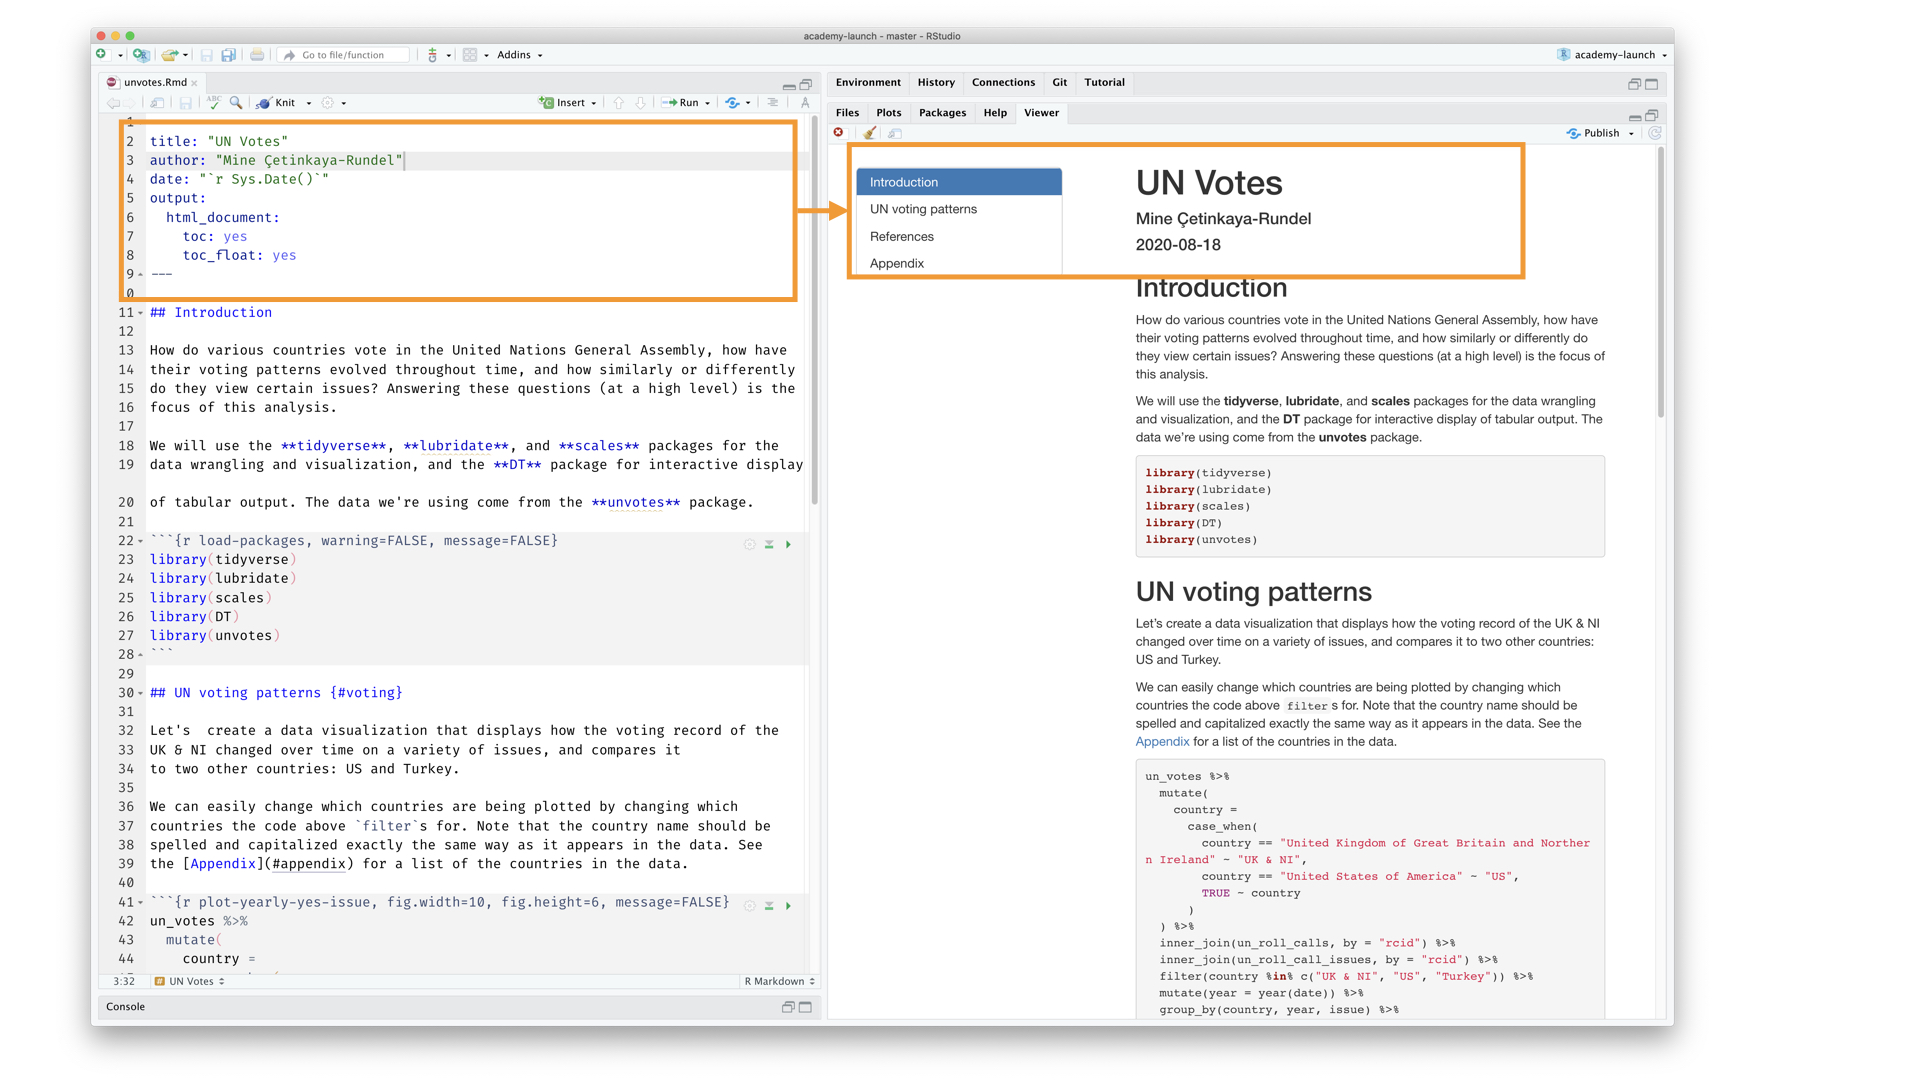
\includegraphics[width=0.9\linewidth]{Images/S1/unvotes/unvotes-14}	
			
			\end{overprint}
		\end{figure}
		
	\end{frame}
	
	%------------------------------------------------------------------%
	
	\begin{frame}
		

		\frametitle{\textbf{Learning Goals}}
		By the end of the course, you will be able to...
		
		\begin{itemize}
			\item gain insight from data
			\item gain insight from data, \structure{reproducibly}
			\item gain insight from data, reproducibly, \structure{using modern programming tools and techniques}
			\item gain insight from data, reproducibly \structure{and collaboratively}, using modern programming tools and techniques
			\item gain insight from data, reproducibly \structure{(with literate programming and version control)} and collaboratively, using modern programming tools and techniques
		\end{itemize}
	\end{frame}
	
		%------------------------------------------------------------------%
	
	\begin{frame}
		
		
		\frametitle{\textbf{Reproducible Data Analysis}}
		
		\begin{itemize}
			\item Near-term goals:
			\begin{itemize}
				\item Are the tables and figures reproducible from the code and data?
				\item Does the code actually do what you think it does?
				\item In addition to what was done, is it clear why it was done?
			\end{itemize}
			\item Long-term goals:
			\begin{itemize}
				\item Can the code be used for other data?
				\item Can you extend the code to do other things?
			\end{itemize}
		\end{itemize}
	\end{frame}

		%------------------------------------------------------------------%

\begin{frame}
	
	
	\frametitle{\textbf{Toolkit for Reproducibility}}
	
	\begin{itemize}
		\item Scriptability $\rightarrow$ R
		\item Literate programming (code, narrative, output in one place) $\rightarrow$ R Markdown
		\item Version control $\rightarrow$ Git / GitHub
	\end{itemize}
\end{frame}
	
			%------------------------------------------------------------------%
	
	\begin{frame}
		
		
		\frametitle{\textbf{R and RStudio}}
		
	\begin{minipage}[t]{0.5\linewidth}
		\vspace{-1em}
		\begin{figure}
			\centering
			
\includegraphics[width=0.2\linewidth]{Images/S1/r-logo}
			\label{fig:r-logo}
		\end{figure}
		
		\begin{itemize}
			\item R is an open-source statistical programming language
			\item R is also an environment for statistical computing and graphics
			\item It's easily extensible with \textit{packages}
		\end{itemize}   
	\end{minipage}%
	\begin{minipage}[t]{0.5\linewidth}
		\vspace{-1em}
	\begin{figure}
		\centering
		
\includegraphics[width=0.4\linewidth]{Images/S1/RStudio_logo}
		\label{fig:rstudiologo}
	\end{figure}
	\vspace{-1em}
	\begin{itemize}
		\item RStudio is a convenient interface for R called an IDE (integrated development environment), e.g. \textit{"I write R code in the RStudio IDE"}
		\item RStudio is not a requirement for programming with R, but it's very commonly used by R programmers and data scientists
	\end{itemize}   

	\end{minipage}
	\end{frame}

		%------------------------------------------------------------------%

\begin{frame}
	
	
	\frametitle{\textbf{R Packages}}
	
	\begin{itemize}
		\item Packages are the fundamental units of reproducible R code. They include reusable R functions, the documentation that describes how to use them, and sample data
		\item As of September 2020, there are over 16,000 R packages available on CRAN (the Comprehensive R Archive Network)
		\item We're going to work with a small (but important) subset of these!
		\item The tidyverse is an opinionated collection of R packages designed for data science.
		\item All packages share an underlying philosophy and a common grammar
	\end{itemize}
\end{frame}

		%------------------------------------------------------------------%

\begin{frame}
	
	
	\frametitle{\textbf{Tour: R and RStudio}}
	
\begin{figure}
	\centering
	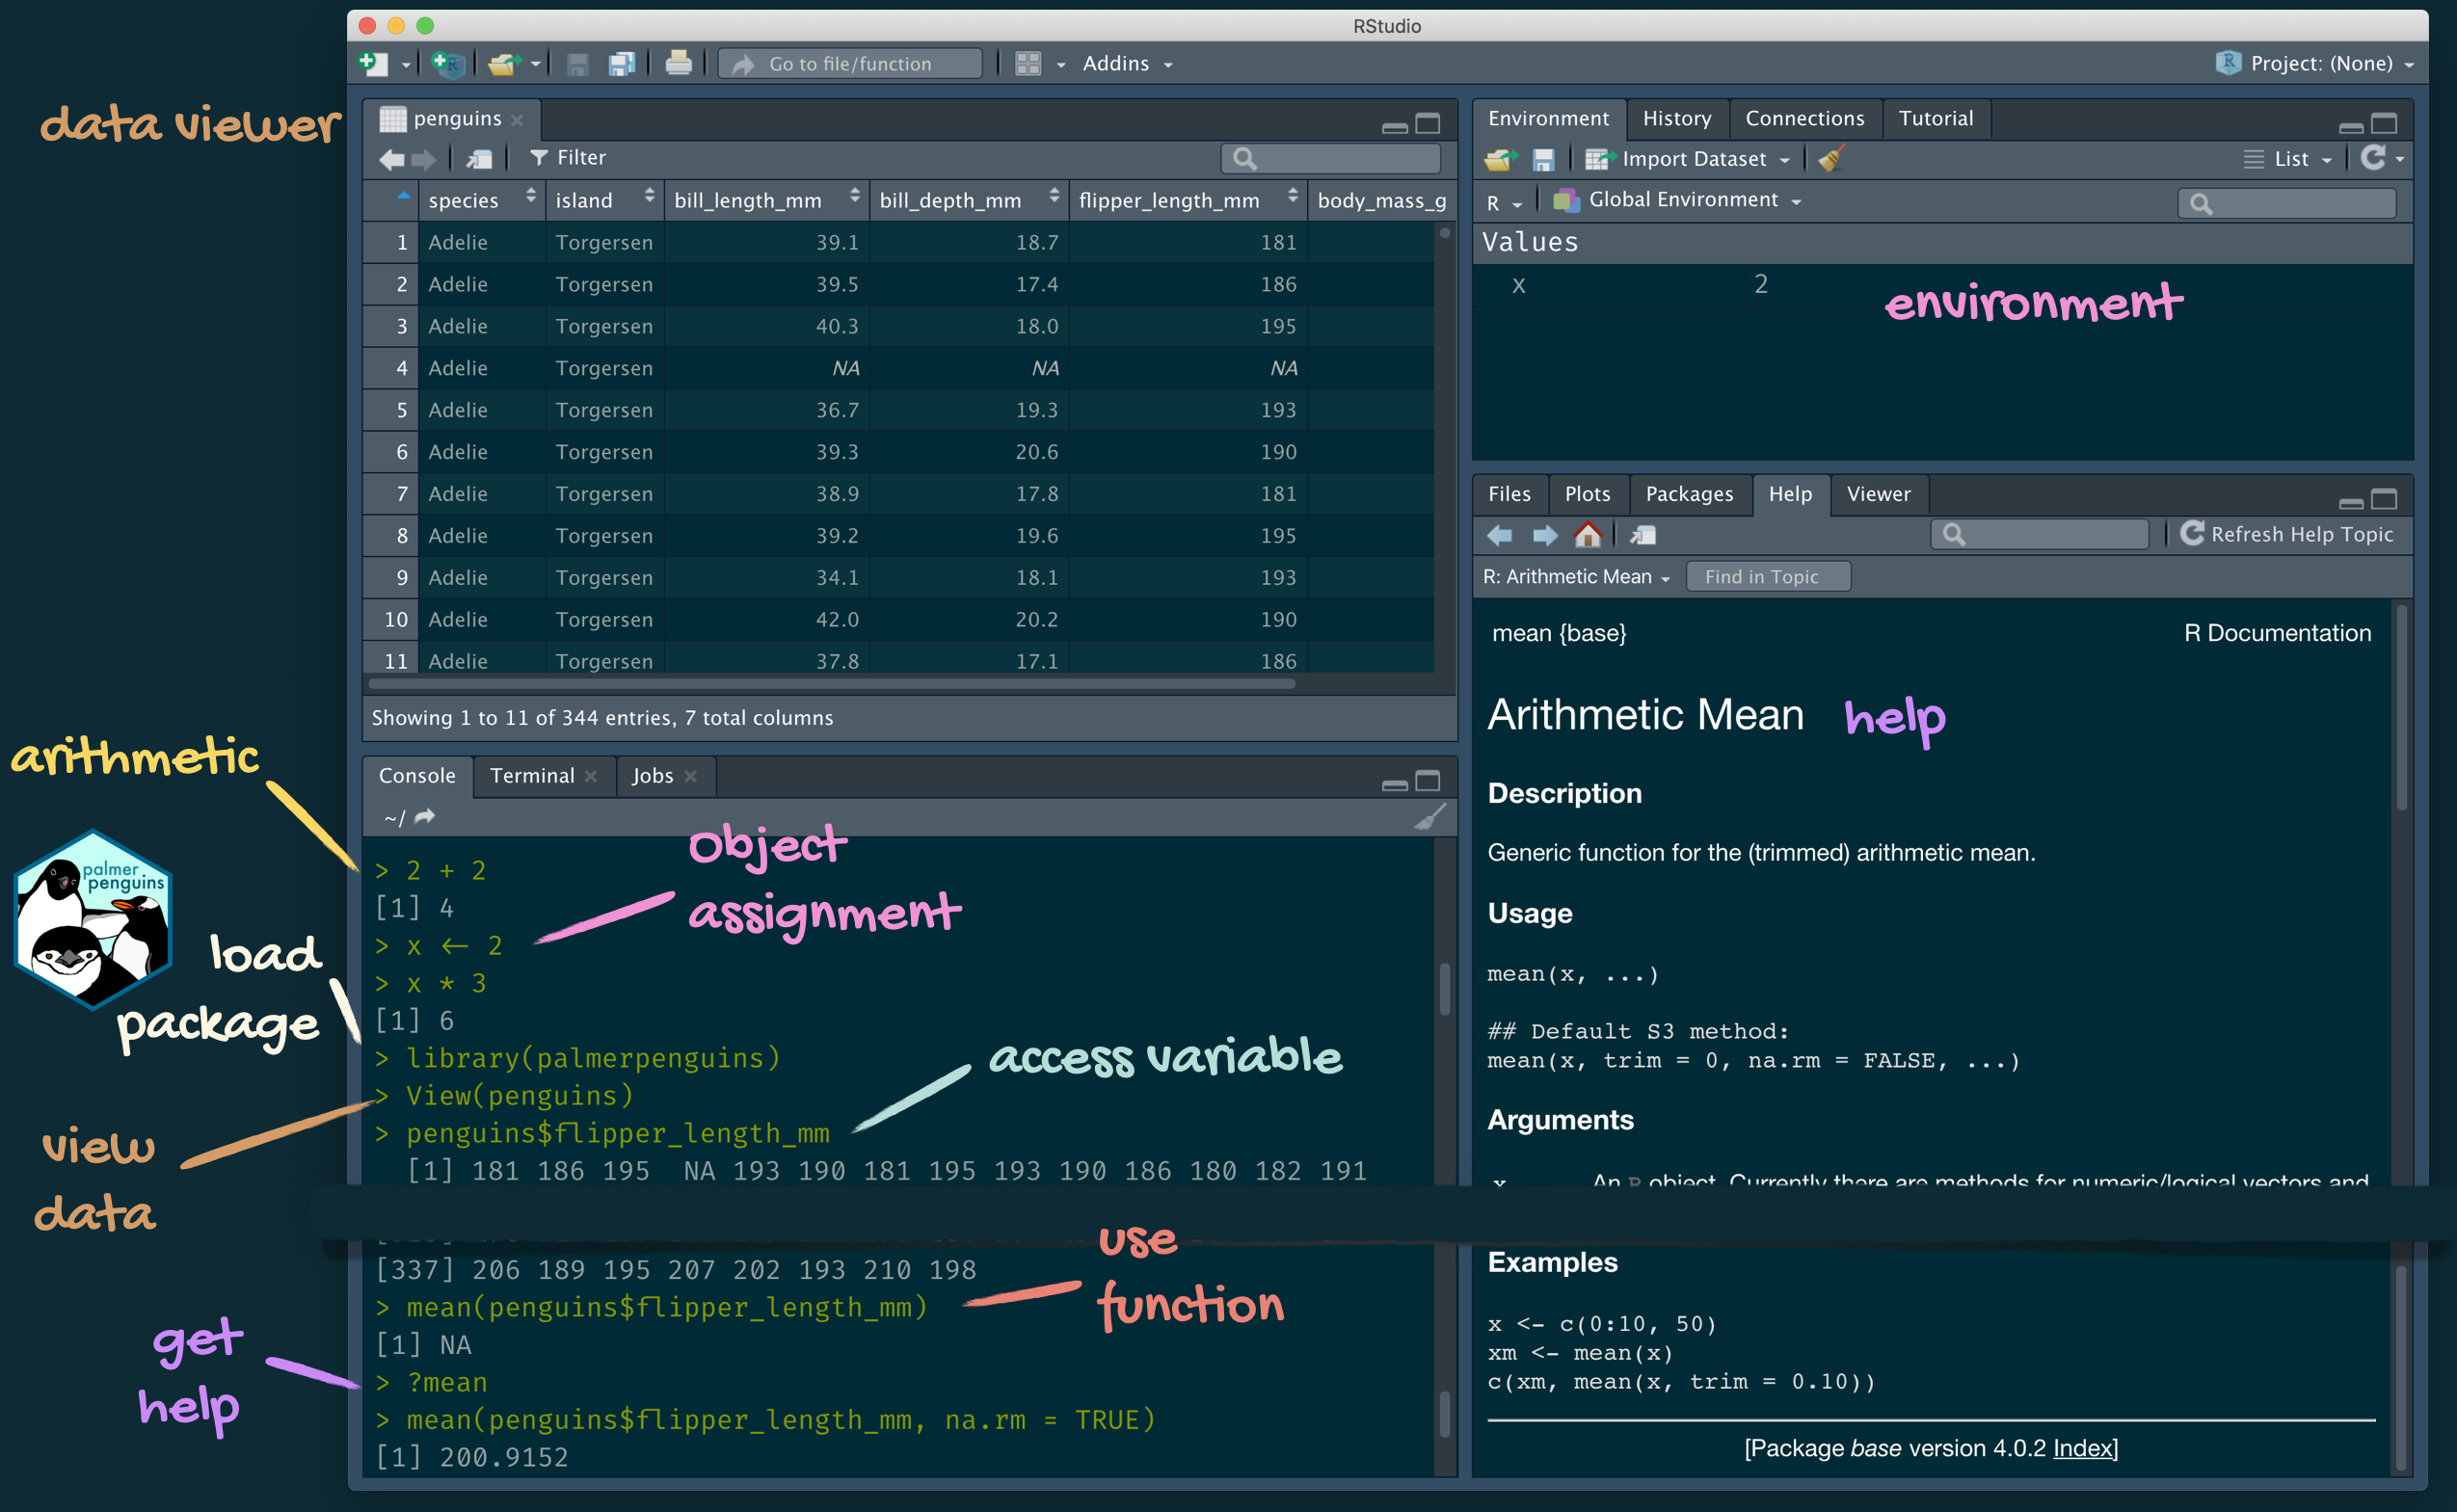
\includegraphics[width=0.75\linewidth]{Images/S1/tour-r-rstudio}
	\label{fig:tour-r-rstudio}
\end{figure}

\end{frame}

		%------------------------------------------------------------------%

\begin{frame}
	
	
	\frametitle{\textbf{Tour: R and RStudio}}
		\small{Functions are (most often) verbs, followed by what they will be applied to in parentheses:
\begin{figure}

	\centering

	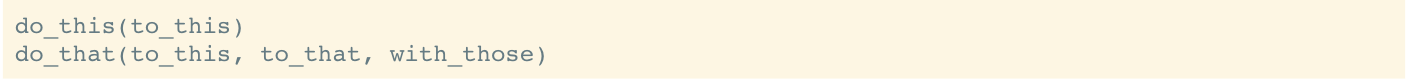
\includegraphics[width=1\linewidth]{Images/S1/code/s1}



\end{figure}
 Packages are installed with the install.packages function and loaded with the library function, once per session:
\begin{figure}
	
	\centering
	

	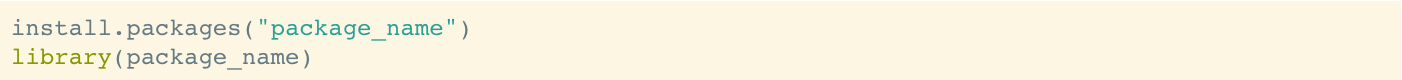
\includegraphics[width=1\linewidth]{Images/S1/code/s2}
	

\end{figure}

 Columns (variables) in data frames are accessed with \$:
\begin{figure}
	
	\centering
	
	
	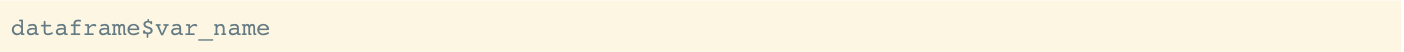
\includegraphics[width=1\linewidth]{Images/S1/code/s3}
	
	
\end{figure}
Object documentation can be accessed with ?}
\begin{figure}
	
	\centering
	
	
	
\includegraphics[width=1\linewidth]{Images/S1/code/s4}
	
	
\end{figure}
	
\end{frame}


%------------------------------------------------------------------%

\begin{frame}
	
	
	\frametitle{\textbf{R Markdown}}
	
\begin{itemize}
	\item rmarkdown and the various packages that support it enable R users to write their code and prose in reproducible computational documents.
	\item We will generally refer to R Markdown documents (with .Rmd extension), e.g. "Do this in your R Markdown document" and rarely discuss loading the rmarkdown package
	\item Fully reproducible reports -- each time you knit the analysis is ran from the beginning
	\item Simple markdown syntax for text
	\item Code goes in chunks, defined by three backticks, narrative goes outside of chunks
\end{itemize}
	
\end{frame}

%------------------------------------------------------------------%

\begin{frame}
	
	
	\frametitle{\textbf{Tour: R Markdown}}
	
	\begin{figure}
		\centering
		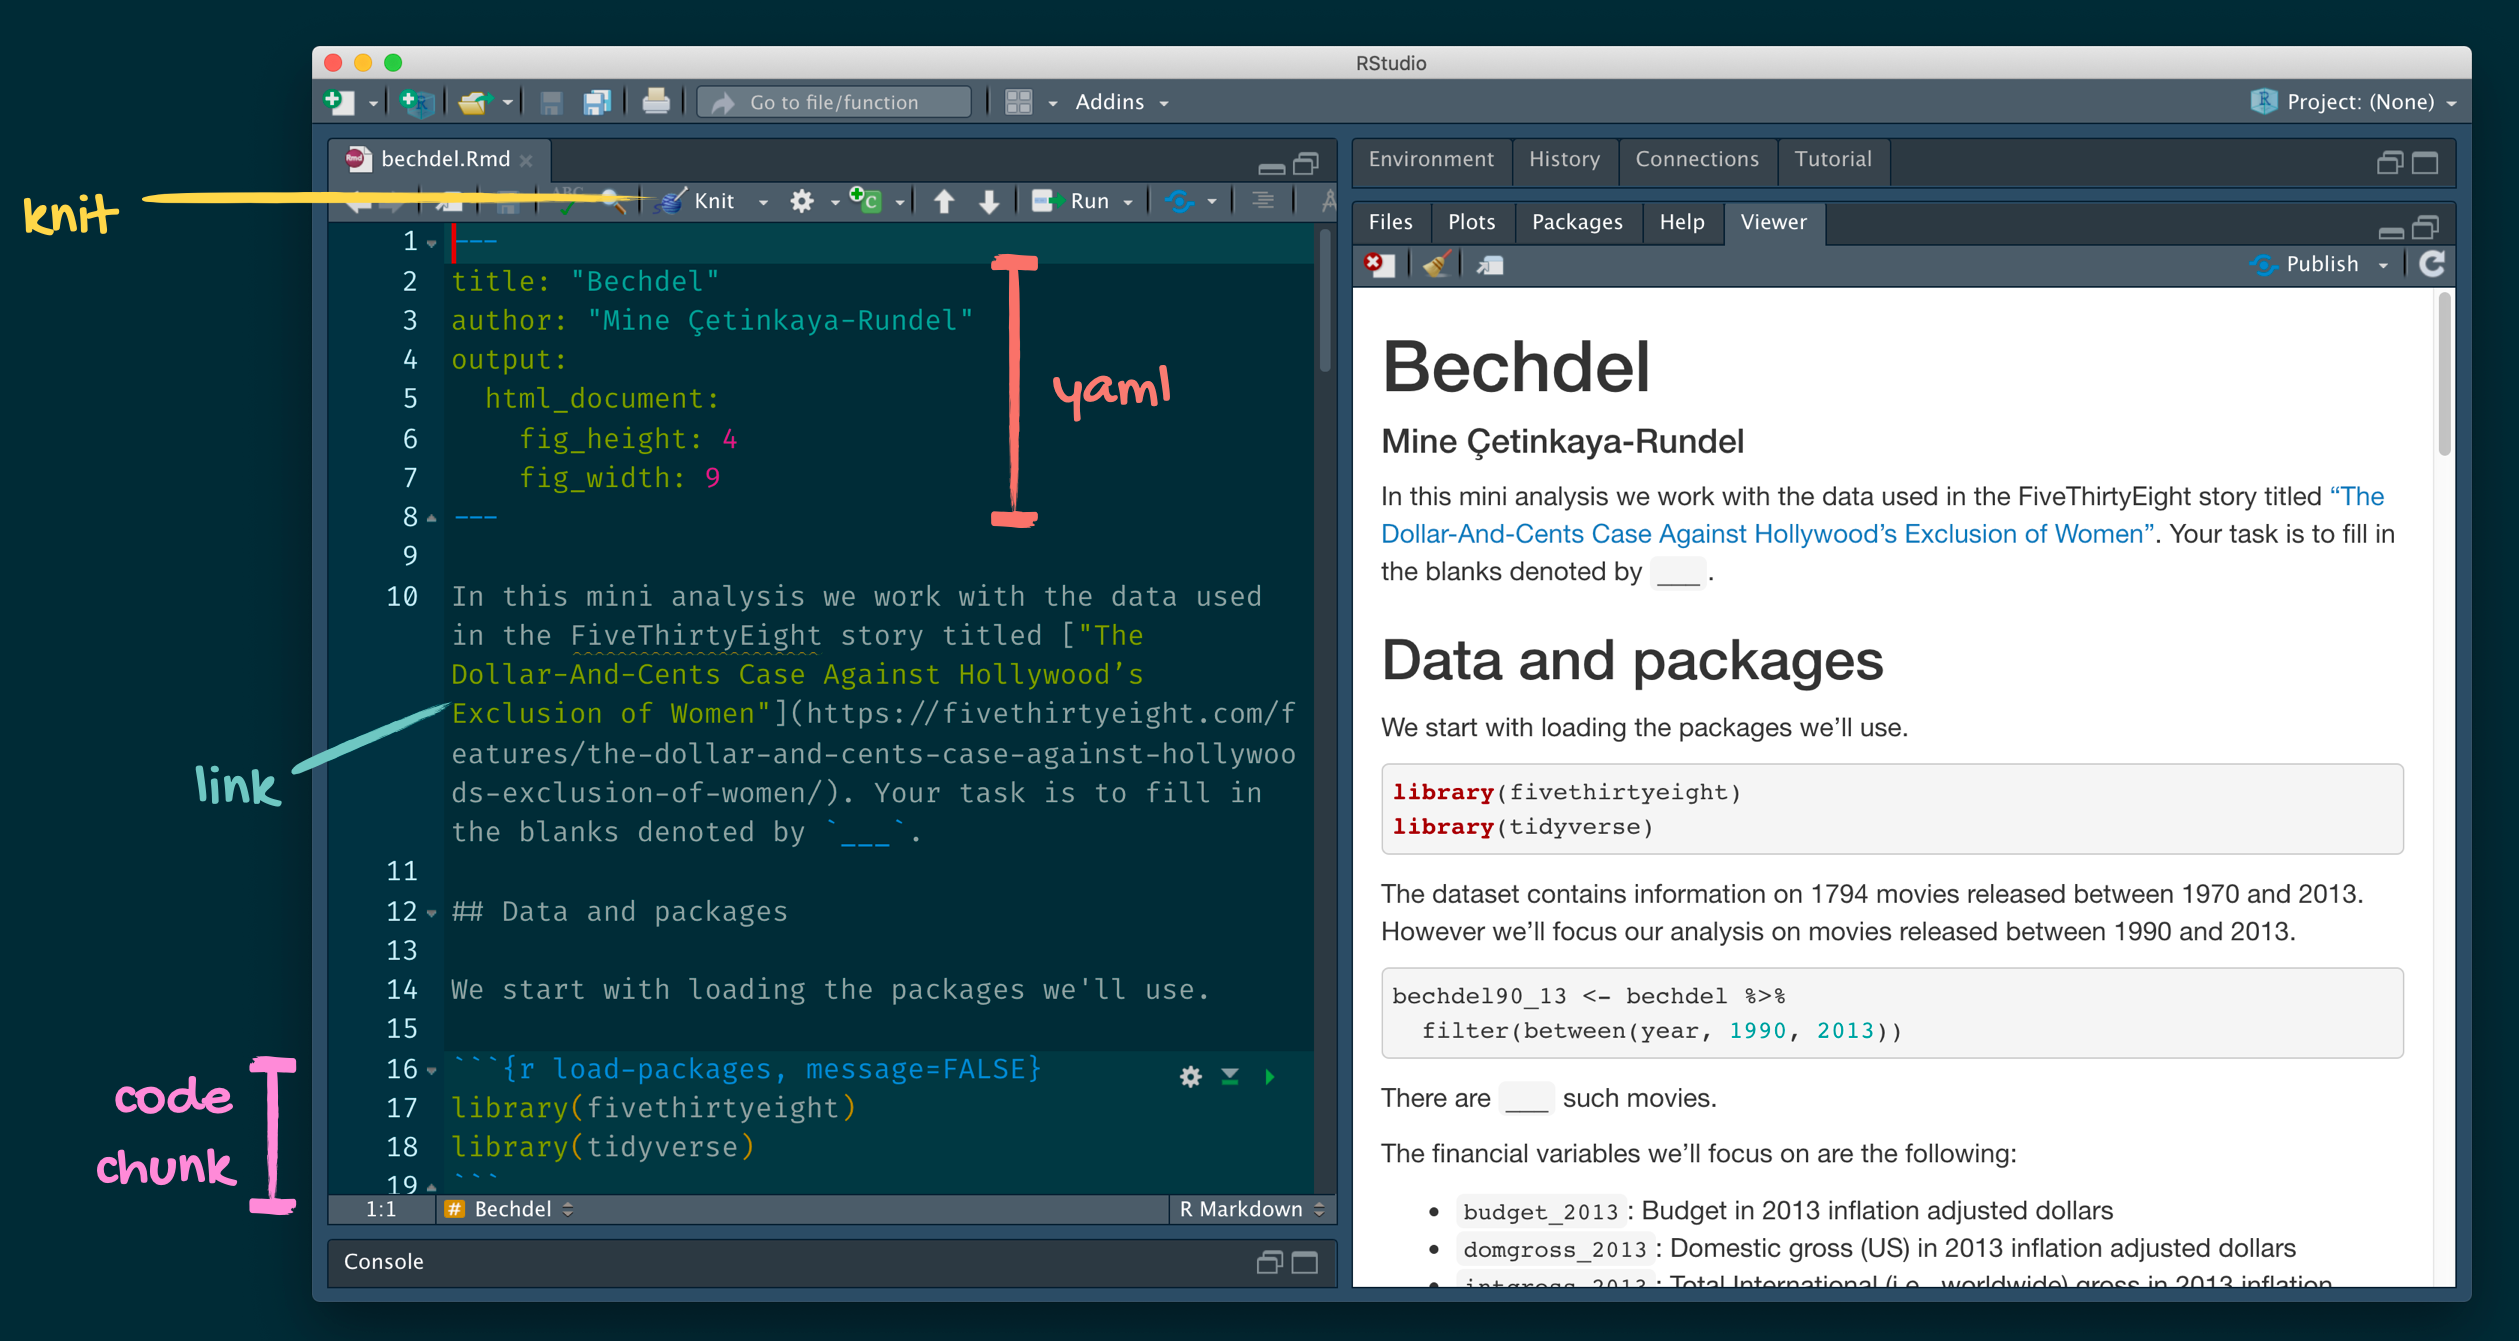
\includegraphics[width=0.9\linewidth]{Images/S1/tour-rmarkdown}
	\end{figure}
	
\end{frame}

%------------------------------------------------------------------%

%------------------------------------------------------------------%


		

	
	%------------------------------------------------------------------%


\begin{frame}
	
	
	\frametitle{\textbf{Version Control and Collaboration}}
	
	\begin{minipage}[t]{0.5\linewidth}
		\vspace{-1em}
		\begin{figure}
			\centering
			
\includegraphics[width=0.2\linewidth]{Images/S1/git-logo}
			\label{fig:r-logo}
		\end{figure}
		
		\begin{itemize}
			\item Git is a version control system -- like ?Track Changes? features from Microsoft Word, on steroids
			\item It's not the only version control system, but it's a very popular one
		\end{itemize}   
	\end{minipage}%
	\begin{minipage}[t]{0.5\linewidth}
		\vspace{-1em}
		\begin{figure}
			\centering
			
\includegraphics[width=0.25\linewidth]{Images/S1/GitHub}
			\label{fig:rstudiologo}
		\end{figure}
		\vspace{-1em}
		\begin{itemize}
			\item GitHub is the home for your Git-based projects on the internet -- like DropBox but much, much better
			\item We will use GitHub as a platform for web hosting and collaboration
		\end{itemize}   
		
	\end{minipage}
\end{frame}

%------------------------------------------------------------------%

\begin{frame}
	
	
	\frametitle{\textbf{Versioning with Human Readable Messages}}
	
	\begin{figure}
		\centering
		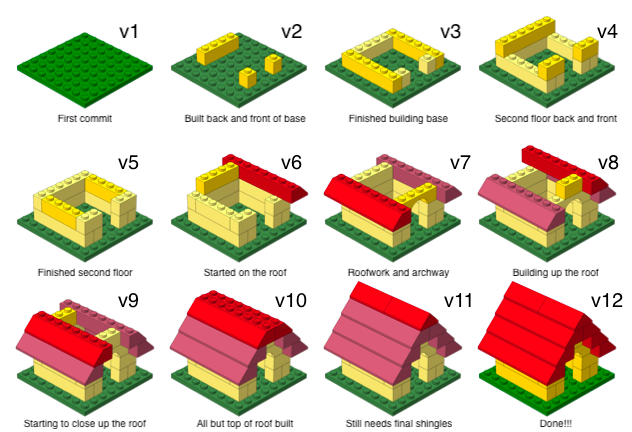
\includegraphics[width=0.67\linewidth]{Images/S1/lego-steps-commit-messages}
	\end{figure}
	
\end{frame}

%------------------------------------------------------------------%
%------------------------------------------------------------------%

\begin{frame}
	\frametitle{\textbf{How Will We Use Git and GitHub?}}
	\begin{figure}
		\vspace{-1em}
		\begin{overprint}
			\onslide<1>\centering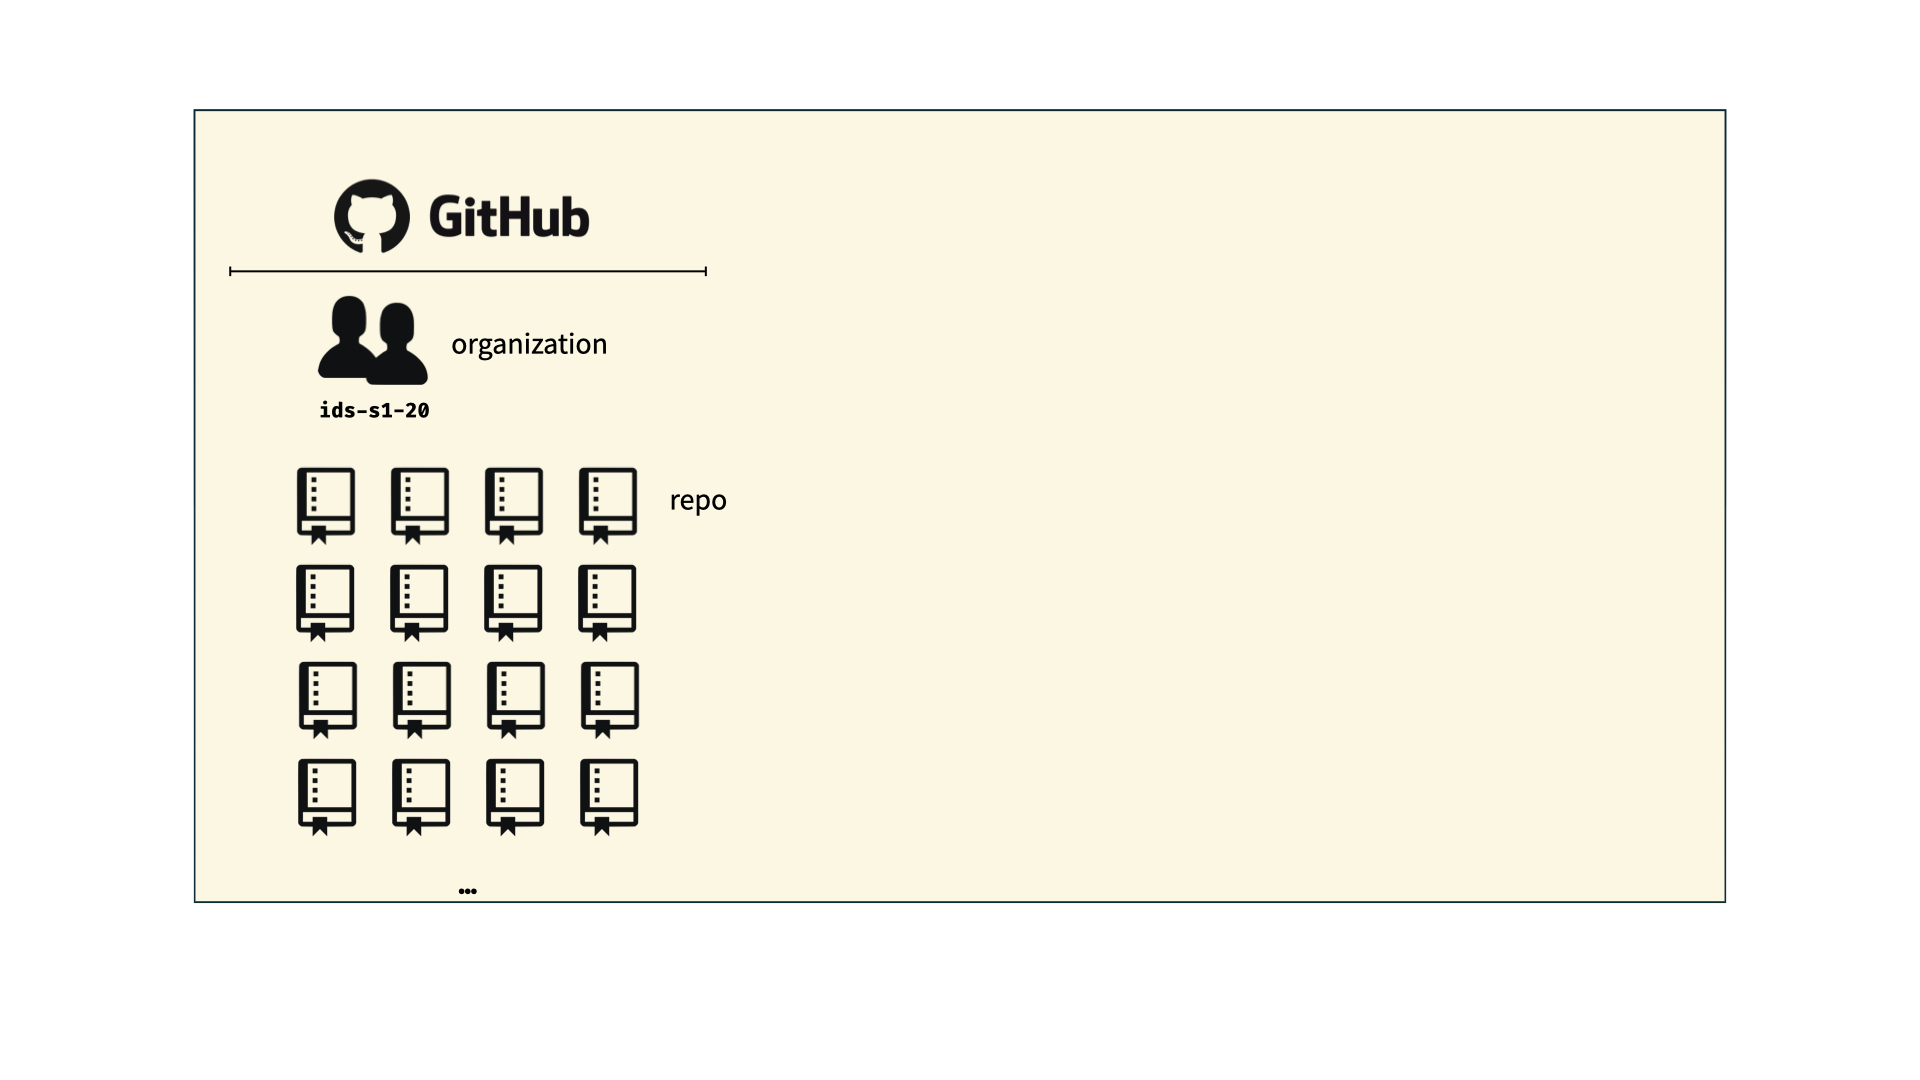
\includegraphics[width=1\linewidth]{Images/S1/whole-game-01}
			\onslide<2>\centering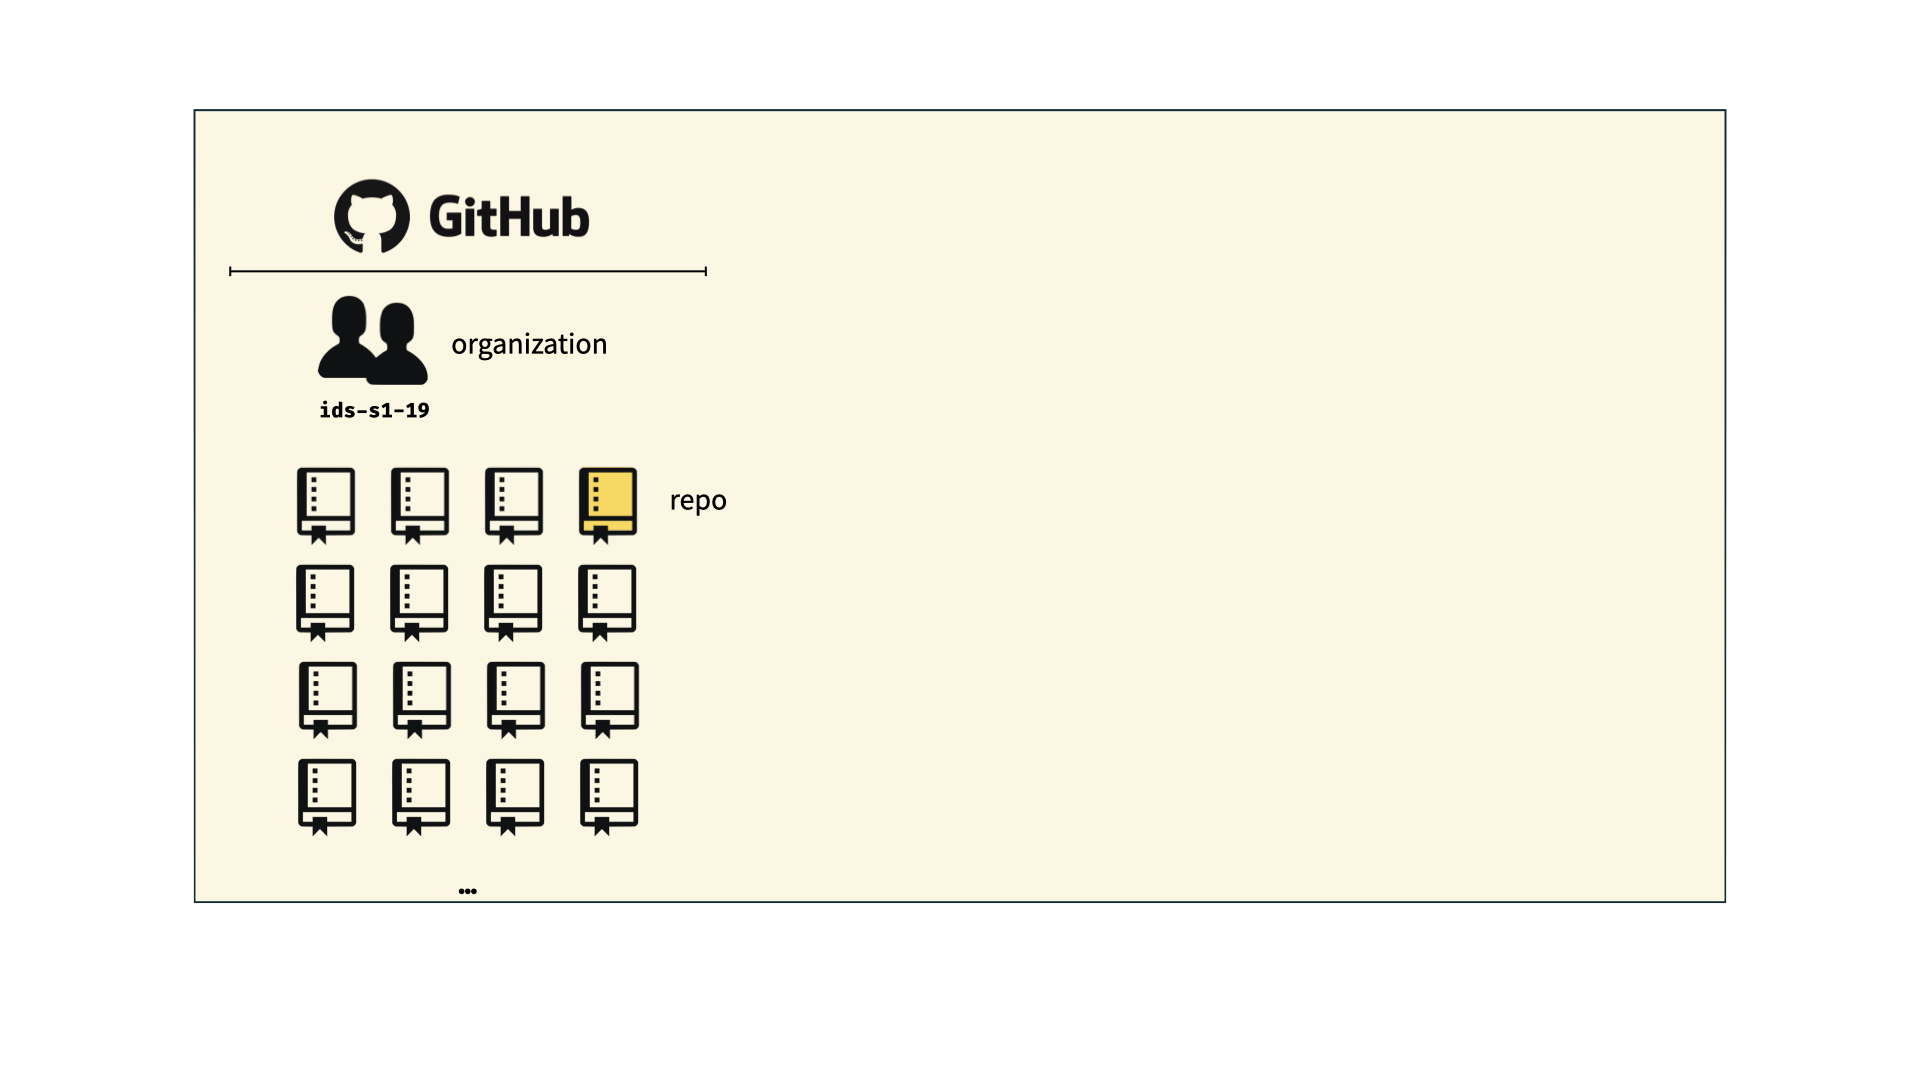
\includegraphics[width=1\linewidth]{Images/S1/whole-game-02}
			\onslide<3>\centering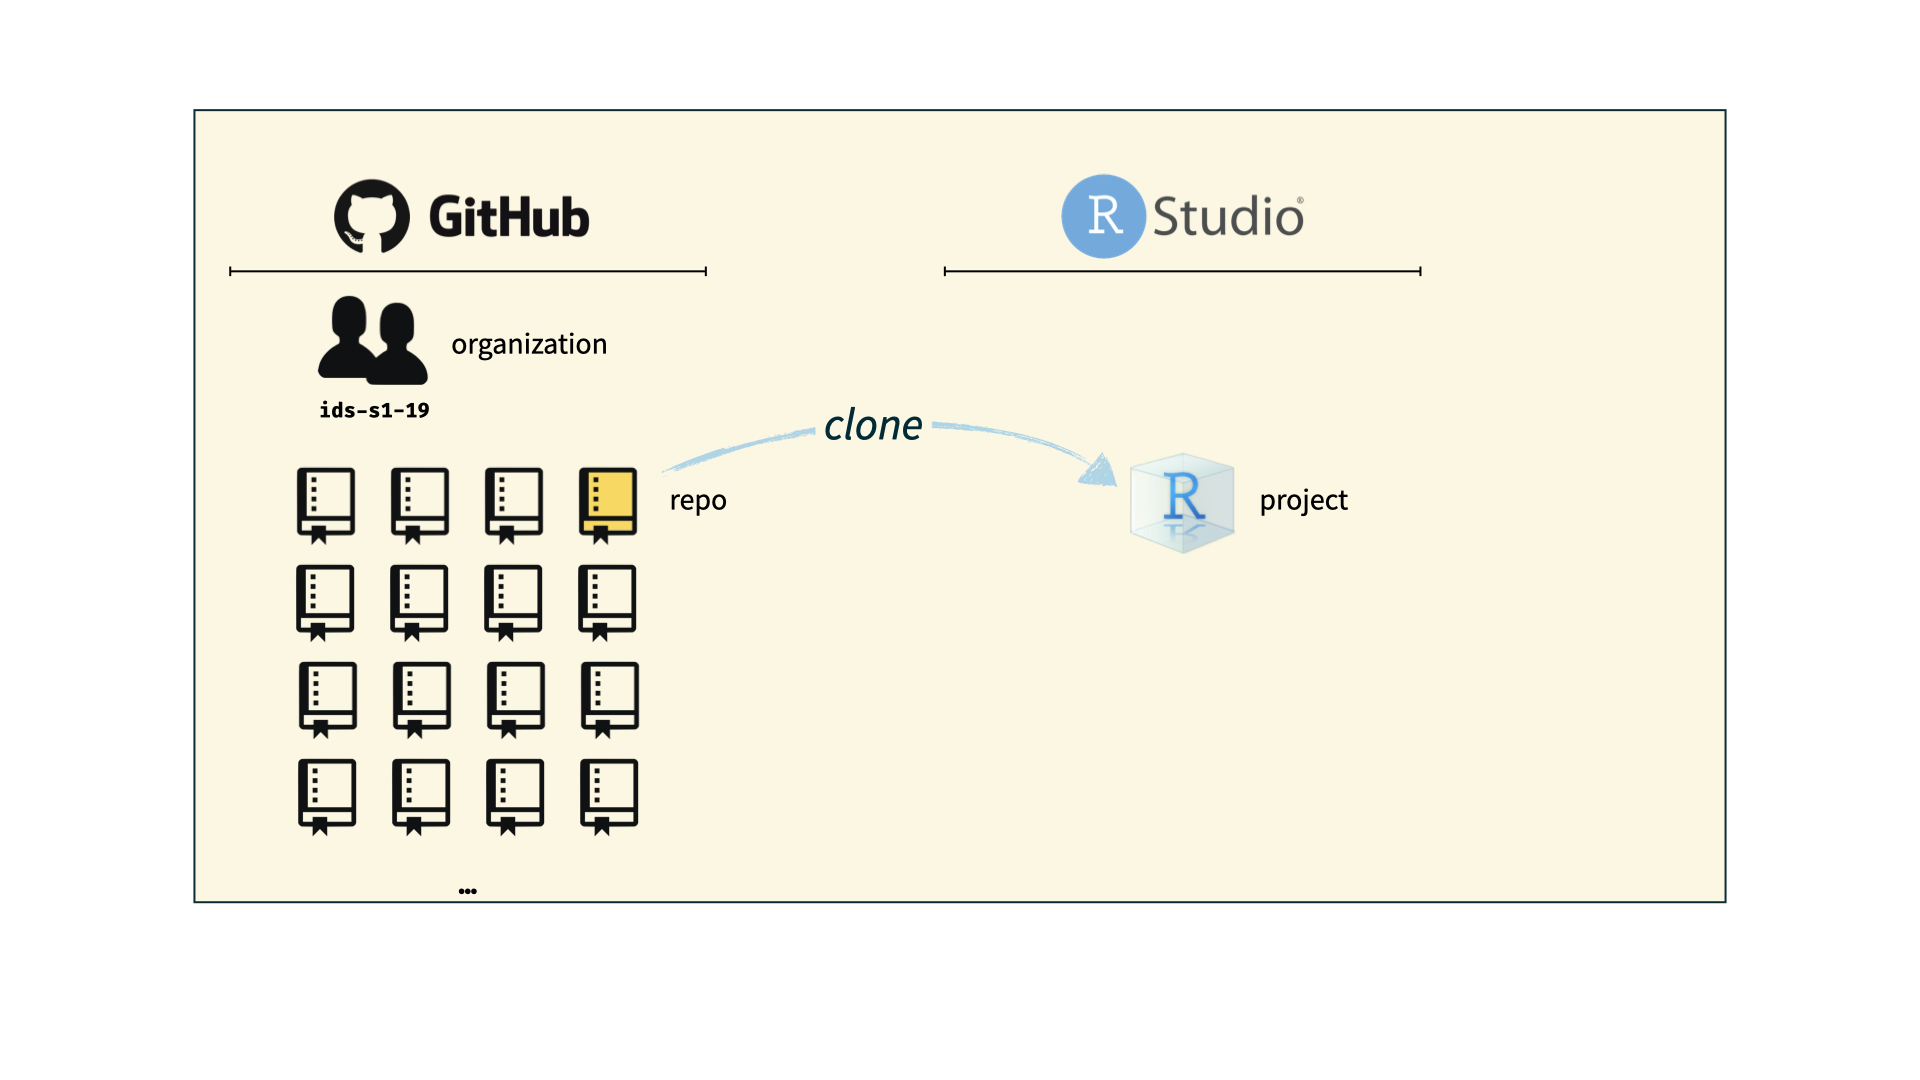
\includegraphics[width=1\linewidth]{Images/S1/whole-game-03}
			\onslide<4>\centering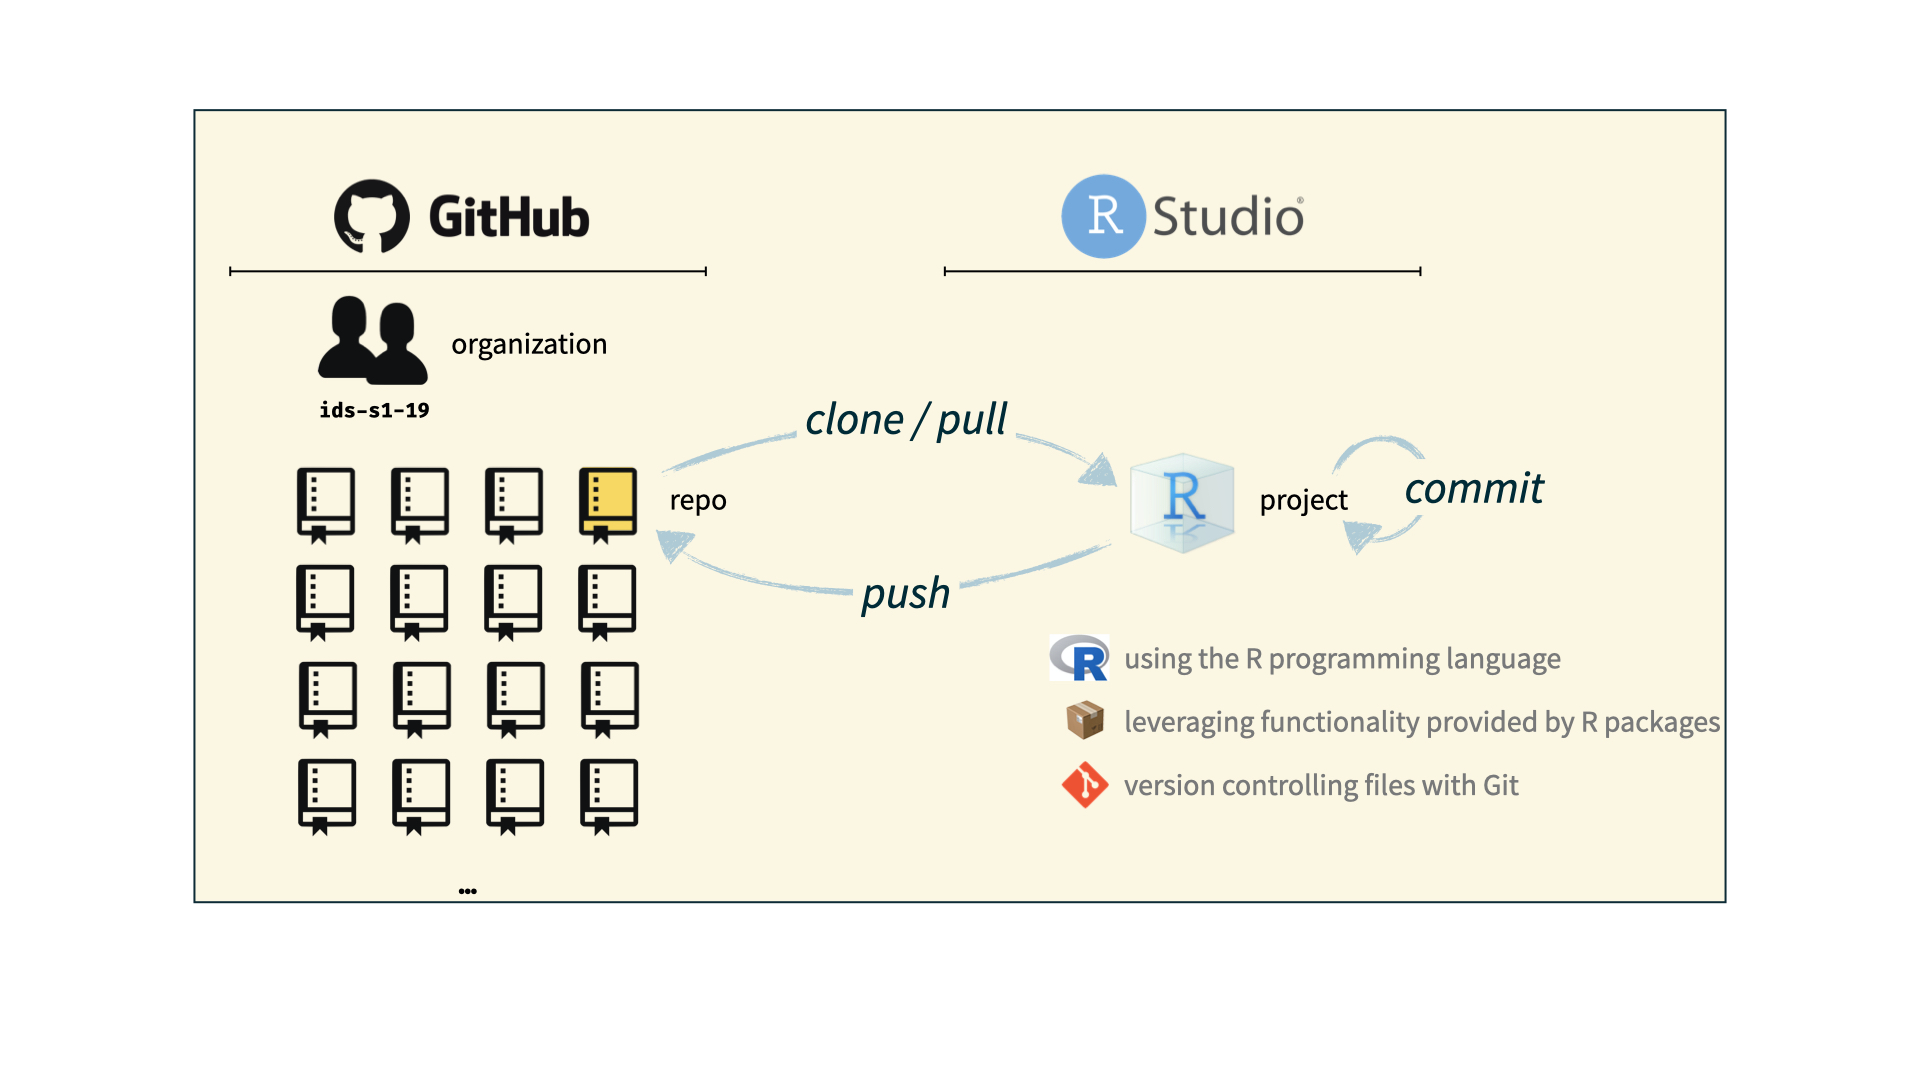
\includegraphics[width=1\linewidth]{Images/S1/whole-game-04}
		\end{overprint}
	\end{figure}
	
\end{frame}

%------------------------------------------------------------------%
%------------------------------------------------------------------%


\end{document}